%%%%%%%%%%%%%%%%%%%%%%%%%%%%%%%%%%%%%%%%%
% baposter Landscape Poster
% LaTeX Template
% Version 1.0 (11/06/13)
%
% baposter Class Created by:
% Brian Amberg (baposter@brian-amberg.de)
%
% This template has been downloaded from:
% http://www.LaTeXTemplates.com
%
% License:
% CC BY-NC-SA 3.0 (http://creativecommons.org/licenses/by-nc-sa/3.0/)
%
%%%%%%%%%%%%%%%%%%%%%%%%%%%%%%%%%%%%%%%%%

%----------------------------------------------------------------------------------------
%	PACKAGES AND OTHER DOCUMENT CONFIGURATIONS
%----------------------------------------------------------------------------------------

\documentclass[landscape,a0paper,fontscale=0.4]{baposter} % Adjust the font scale/size here

\hyphenation{op-tical net-works semi-conduc-tor}
\usepackage{url}
\usepackage{amsmath}
\usepackage{listings}
\usepackage{algorithm}
\usepackage{algorithmic}
\usepackage{lipsum}
\usepackage{xcolor}
\usepackage{bookmark}
\def\code#1{\texttt{#1}}

\usepackage{graphicx} % Required for including images
\graphicspath{{figures/}} % Directory in which figures are stored

\usepackage{amsmath} % For typesetting math
\usepackage{amssymb} % Adds new symbols to be used in math mode

\usepackage{booktabs} % Top and bottom rules for tables
\usepackage{enumitem} % Used to reduce itemize/enumerate spacing
\usepackage{palatino} % Use the Palatino font
\usepackage[font=small,labelfont=bf]{caption} % Required for specifying captions to tables and figures
\usepackage{nth}
\usepackage{subcaption}
\usepackage{multicol} % Required for multiple columns
\setlength{\columnsep}{1.5em} % Slightly increase the space between columns
\setlength{\columnseprule}{0mm} % No horizontal rule between columns

\usepackage{tikz} % Required for flow chart
\usetikzlibrary{shapes,arrows} % Tikz libraries required for the flow chart in the template

\newcommand{\compresslist}{ % Define a command to reduce spacing within itemize/enumerate environments, this is used right after \begin{itemize} or \begin{enumerate}
\setlength{\itemsep}{1pt}
\setlength{\parskip}{0pt}
\setlength{\parsep}{0pt}
}

\definecolor{lightblue}{rgb}{0.145,0.6666,0.9} % Defines the color used for content box headers
\definecolor{black}{rgb}{0.3,0.3,0.3}
\begin{document}

\begin{poster}
{
headerborder=closed, % Adds a border around the header of content boxes
colspacing=0.7em, % Column spacing
bgColorOne=white, % Background color for the gradient on the left side of the poster
bgColorTwo=white, % Background color for the gradient on the right side of the poster
borderColor=lightblue, % Border color
headerColorOne=black, % Background color for the header in the content boxes (left side)
headerColorTwo=lightblue, % Background color for the header in the content boxes (right side)
headerFontColor=white, % Text color for the header text in the content boxes
boxColorOne=white, % Background color of the content boxes
textborder=roundedleft, % Format of the border around content boxes, can be: none, bars, coils, triangles, rectangle, rounded, roundedsmall, roundedright or faded
eyecatcher=true, % Set to false for ignoring the left logo in the title and move the title left
headerheight=0.08\textheight, % Height of the header
headershape=roundedright, % Specify the rounded corner in the content box headers, can be: rectangle, small-rounded, roundedright, roundedleft or rounded
headerfont=\Large\bf\textsc, % Large, bold and sans serif font in the headers of content boxes
%textfont={\setlength{\parindent}{1.5em}}, % Uncomment for paragraph indentation
linewidth=1.5pt, % Width of the border lines around content boxes
columns =3
}
%----------------------------------------------------------------------------------------
%	TITLE SECTION 
%----------------------------------------------------------------------------------------
%
{
\includegraphics[height=11em]{wits.jpg}} % First university/lab logo on the left
{\bf\textsc{Image Compression based on Non-Parametric Sampling in Noisy Environments}\vspace{0.3em}} % Poster title
{\textsc{Kishan Narotam \& Nitesh Nana \hspace{12pt} {\small School of Electrical \& Information Engineering, University of the Witwatersrand}}} % Author names and institution
	{
\includegraphics[height=11em]{EIE.pdf}} % Second university/lab logo on the right

%----------------------------------------------------------------------------------------
%----------------------------------------------------------------------------------------
%	LEFT COLUMN
%----------------------------------------------------------------------------------------
%----------------------------------------------------------------------------------------

%----------------------------------------------------------------------------------------
%	OBJECTIVES
%----------------------------------------------------------------------------------------

\headerbox{Objectives}{name=objectives,column=0,row=0}{
To develop a robust scheme for image compression involving the creation of holes, encoding, transmitting and consequently receiving, decoding and filling these holes. 
\begin{itemize}\compresslist
	\vspace{-0.4em}
	\item Creating holes in an image
	\item Encode and transmit the image
	\item Simulate a noisy channel in order to introduce errors
	\item Identifying and filling the holes appropriately.
\end{itemize}

}


%----------------------------------------------------------------------------------------
%	SYSTEM DESIGN
%----------------------------------------------------------------------------------------

\headerbox{System Design}{name=systemDesign,column=0,below=objectives}{ % This block's bottom aligns with the bottom of the conclusion block
	
	\begin{center}
		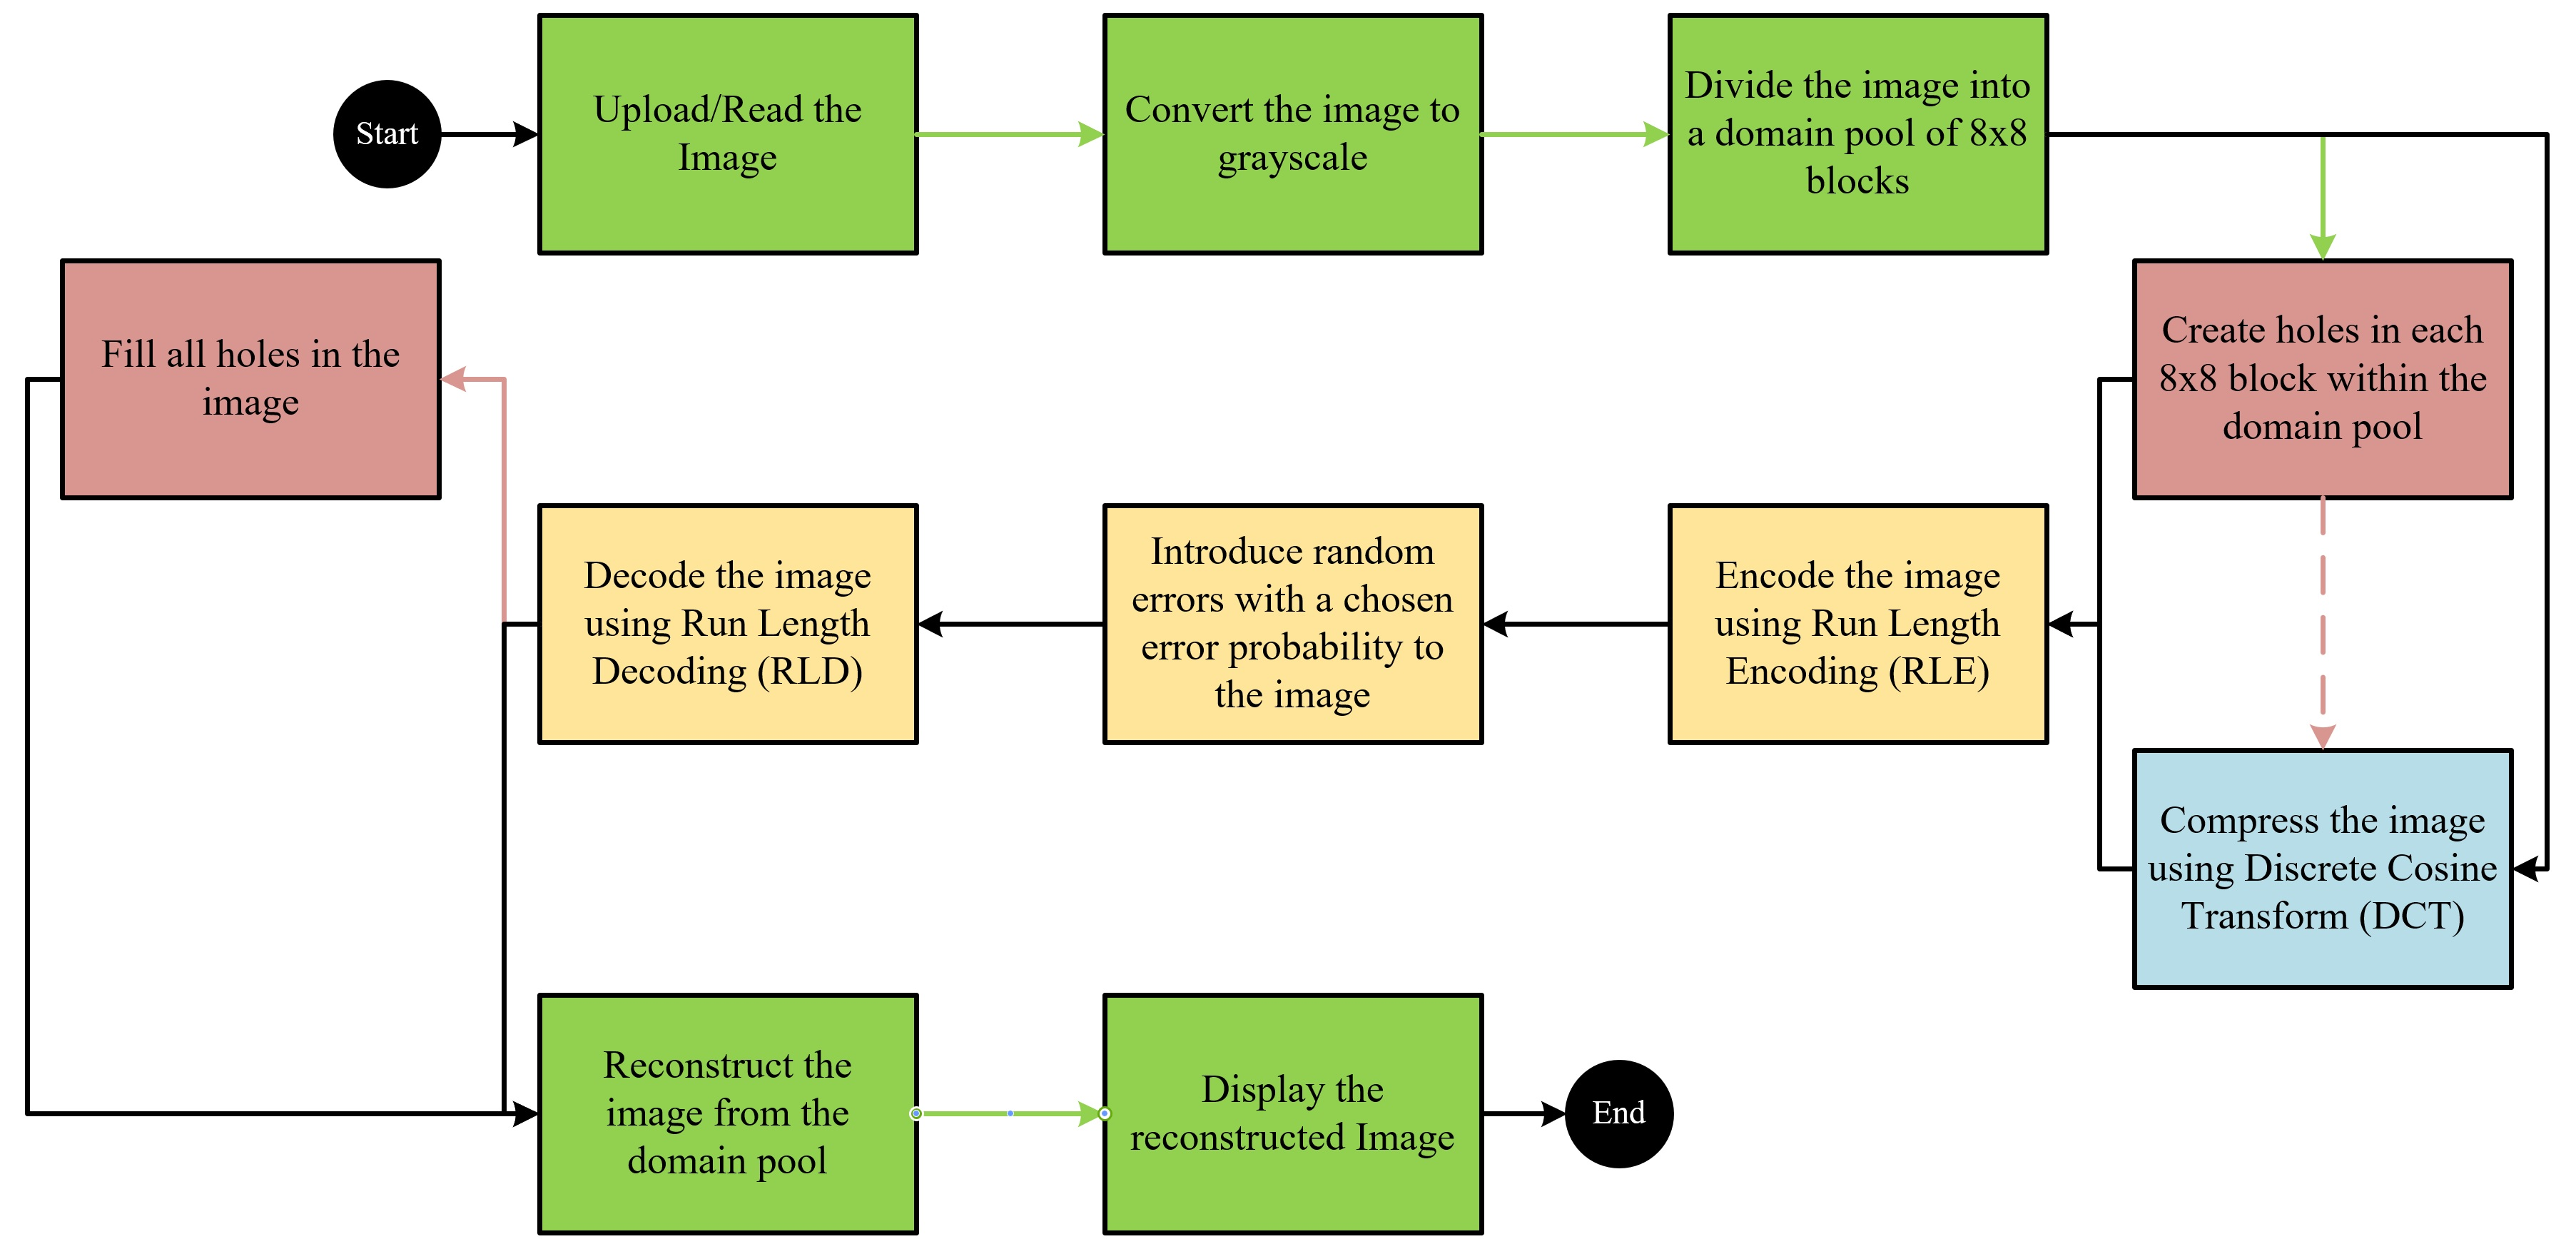
\includegraphics[width=1\linewidth]{BlockDiagram}
		\captionof{figure}{Image compression implementation overview}
	\end{center}
	
}

%----------------------------------------------------------------------------------------
%	ALGORITHMS
%----------------------------------------------------------------------------------------

\headerbox{Algorithms}{name=systemdesign,column=0,below=systemDesign, above=bottom}{ % This block's bottom aligns with the bottom of the conclusion block
	
\begin{algorithm}[H]
\caption{High-level algorithm for creating holes in \code{8x8} blocks}
\label{alg: Creating Holes}
\begin{algorithmic}
\FOR{every block in the domain pool}
	\STATE Go to \code{2x2} square in \code{8x8} block
	\STATE Calculate average of pixels in \code{2x2}
	\STATE
	\FOR{every pixel in the \code{2x2}}
		\STATE Check Chebyshev distance between pixels and average 
	\ENDFOR
	\IF{distance between the average and each pixel $<$ 6}
		\STATE Go to \code{4x4} square in \code{8x8} block
		\STATE Calculate average of pixels of \code{4x4}
		\STATE
		\FOR{every pixel in the \code{4x4}}
			\STATE Check Chebyshev distance between each pixel
		\ENDFOR
		\IF{distance between the average and each pixel $<$ 6}
			\STATE Go to \code{6x6} square in \code{8x8} block
			\STATE Calculate average of pixels of \code{6x6}
			\STATE
			\FOR{every pixel in the \code{6x6}}
				\STATE Check Chebyshev distance between each pixel and average value 
			\ENDFOR
			\IF{distance between average and each pixel $<$ 6}
				\STATE Create hole in \code{6x6}
			\ELSE
				\STATE Create hole in \code{4x4}
			\ENDIF
			\STATE
		\ELSE
			\STATE Create hole in \code{2x2}
	\ENDIF
	\ELSE
		\STATE Move to next block in domain pool
	\ENDIF
\ENDFOR
\end{algorithmic}
\end{algorithm}


	
}

%----------------------------------------------------------------------------------------
%----------------------------------------------------------------------------------------
%	MIDDLE COLUMN
%----------------------------------------------------------------------------------------
%----------------------------------------------------------------------------------------
%----------------------------------------------------------------------------------------
%	RESULTS: PROCESSING
%----------------------------------------------------------------------------------------

\headerbox{Results: Processing}{name=resultsProcessing,column=1,row=0}{

In the figures below, the various steps and processes that the image goes through can be seen.

}

%----------------------------------------------------------------------------------------
%	RESULTS: SIMULATION
%----------------------------------------------------------------------------------------
\headerbox{Results: Simulation}{name=resultsSimulation,column=1, below=resultsProcessing}{
Figure~\ref{fig: CR} and the subsequent sub-figures test the created \emph{Holes} algorithm on different images. Pattern images are chosen for the repetitive colour and smooth features; landscape images are chosen for the texture features and intense detail; high contrast images are chosen for its combination of both repetitive colour, smooth and texture features. 
\vspace{-1em}
\begin{figure}[H]
\centering
	\begin{subfigure}{0.3\textwidth} % width of left subfigure
		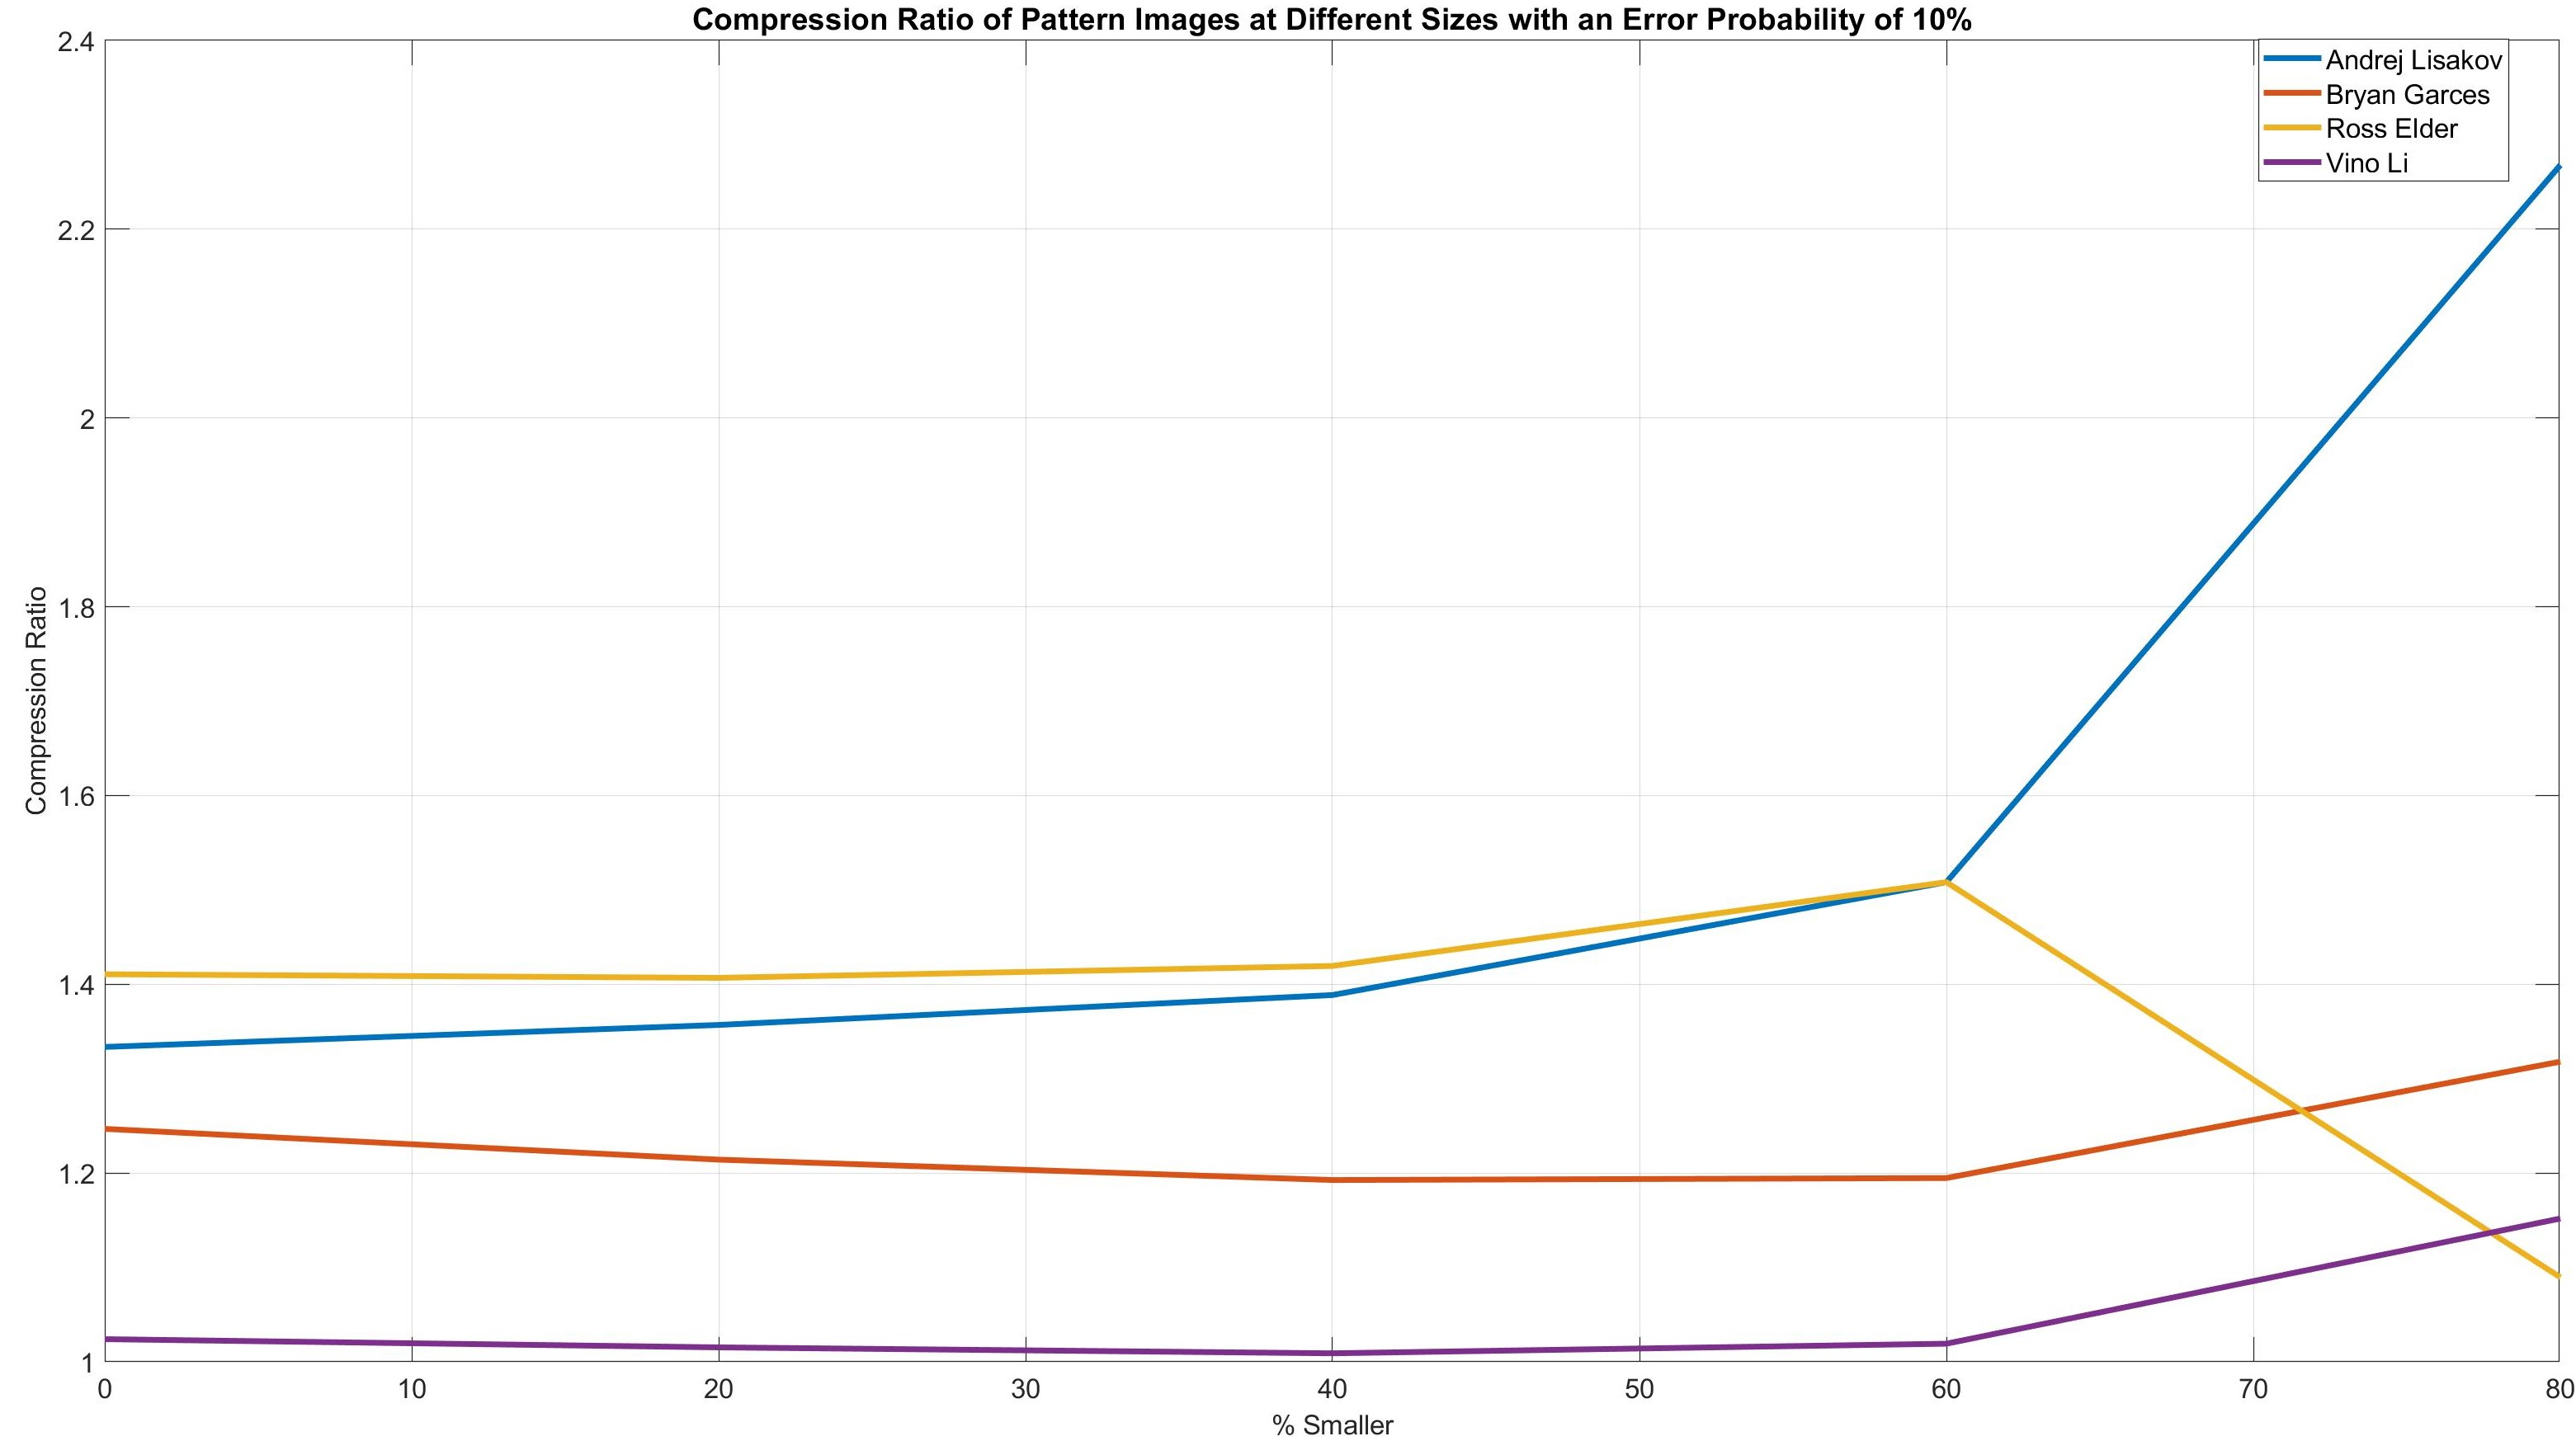
\includegraphics[scale=0.055]{PatternGraph}
		\caption{Pattern Images} % subcaption
	\end{subfigure}
	\vspace{1em} % here you can insert horizontal or vertical space
	\begin{subfigure}{0.3\textwidth} % width of right subfigure
		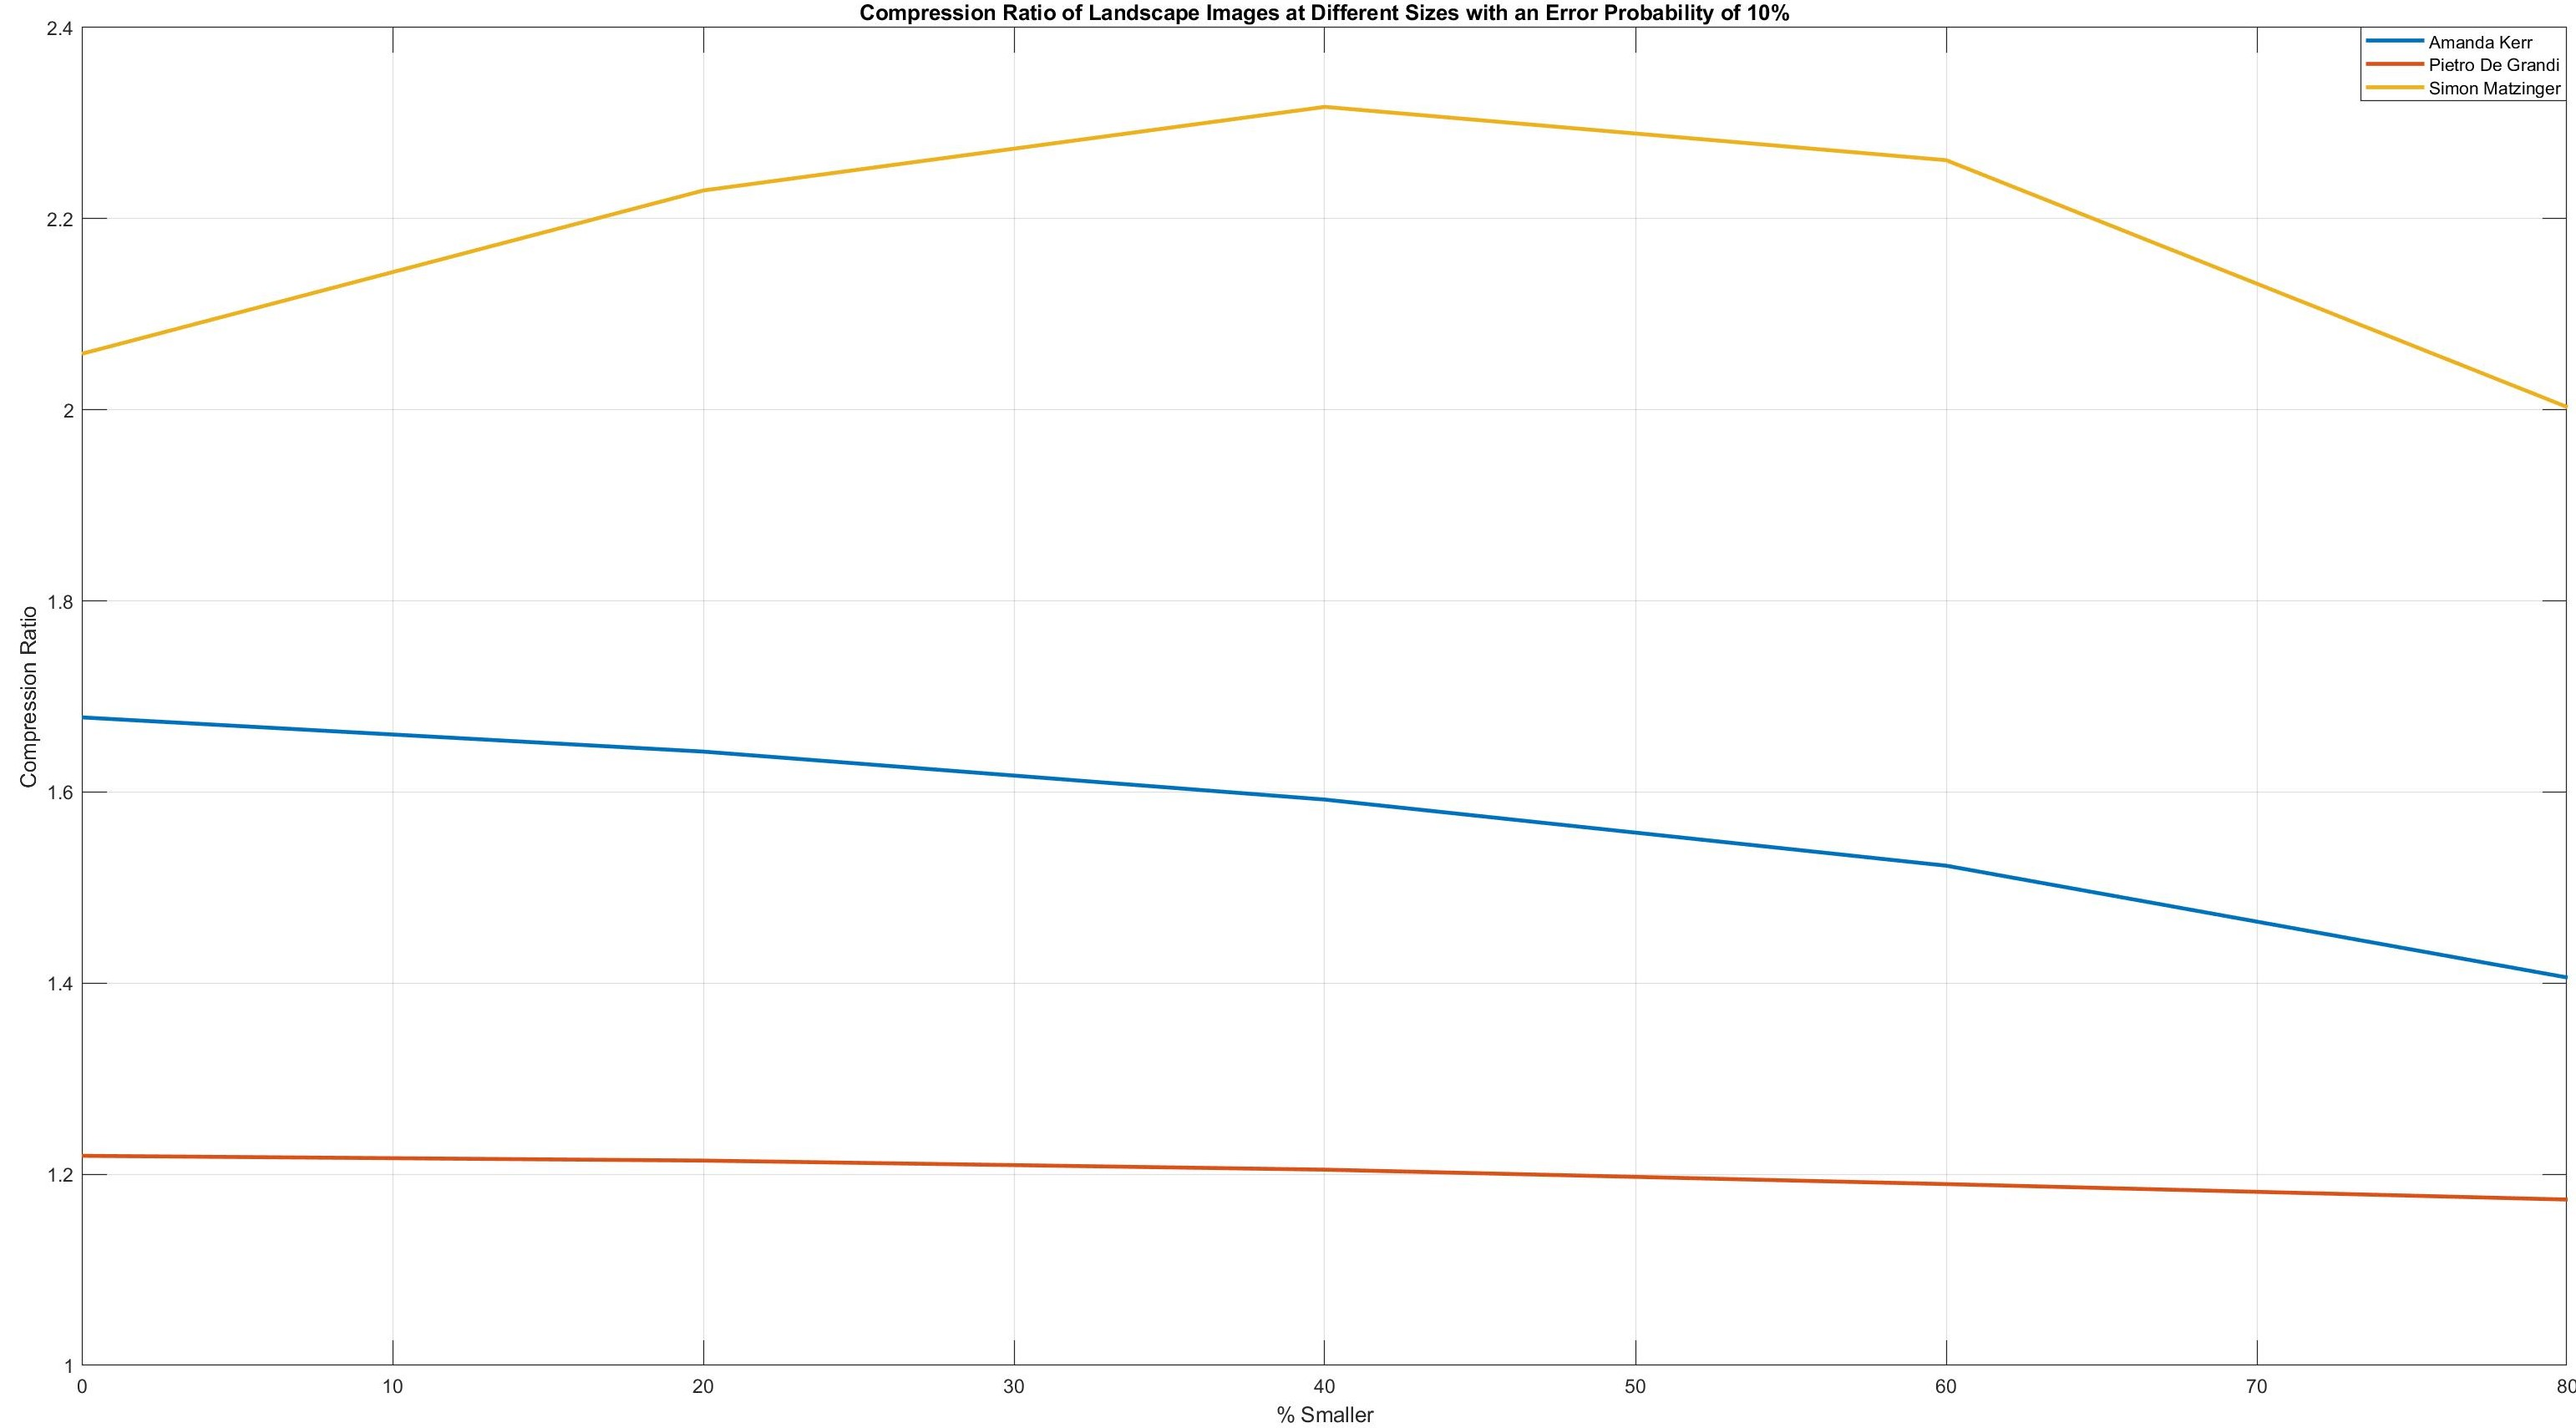
\includegraphics[scale=0.055]{LandscapeGraph}
		\caption{Landscape Images} % subcaption
	\end{subfigure}
	\begin{subfigure}{0.3\textwidth} % width of right subfigure
		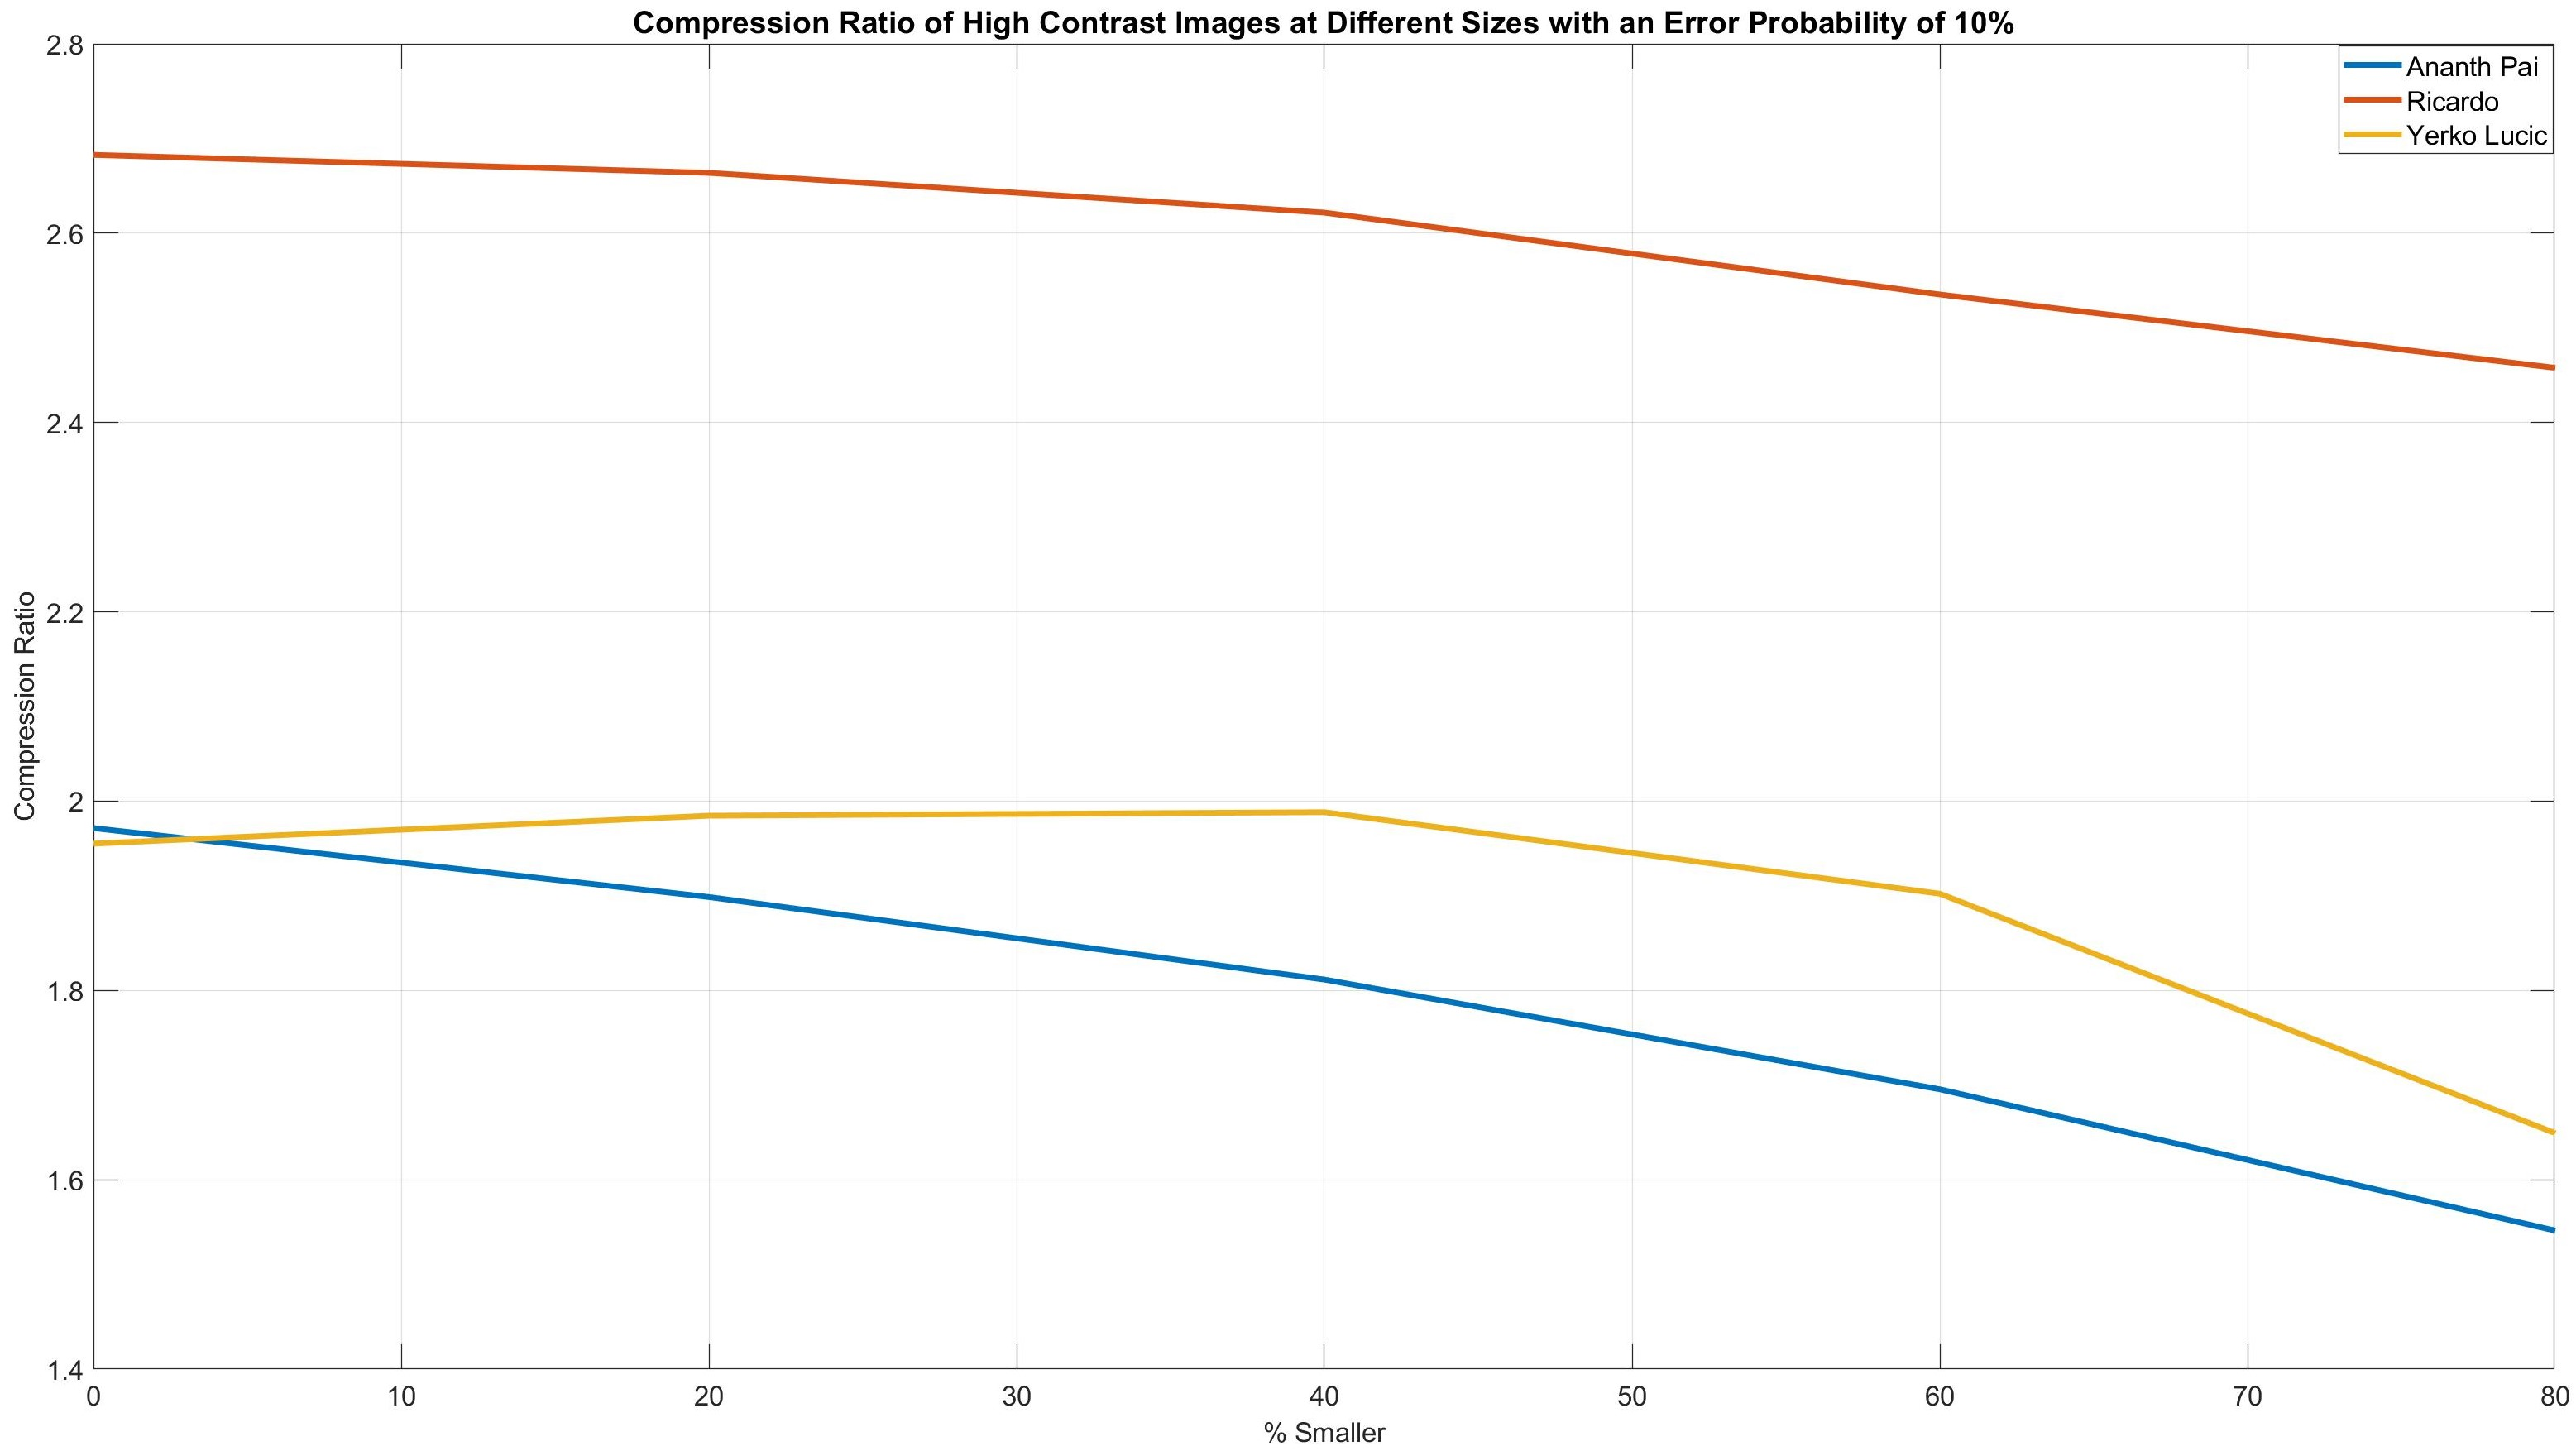
\includegraphics[scale=0.055]{HighContrastGraph}
		\caption{High Contrast Images} % subcaption
	\end{subfigure}
	\vspace{-2em}
	\caption{Compression Ratio vs Same Image at Different Sizes}
	\label{fig: CR} % caption for whole figure
\end{figure}

An error analysis is carried out on the different image types calculating the peak signal-to-noise ratio (PSNR) and mean squared error (MSE) of the reconstructed images. The PSNR is a dimensionless number expressed on a logarithmic decibel scale, to identify the perceived errors noticeable by the human vision. The MSE is the cumulative squared error of the compressed image against the original image~\cite{Error}.
\vspace{-1em}
\begin{figure}[H]
\centering
	\begin{subfigure}{0.4\textwidth} % width of left subfigure
		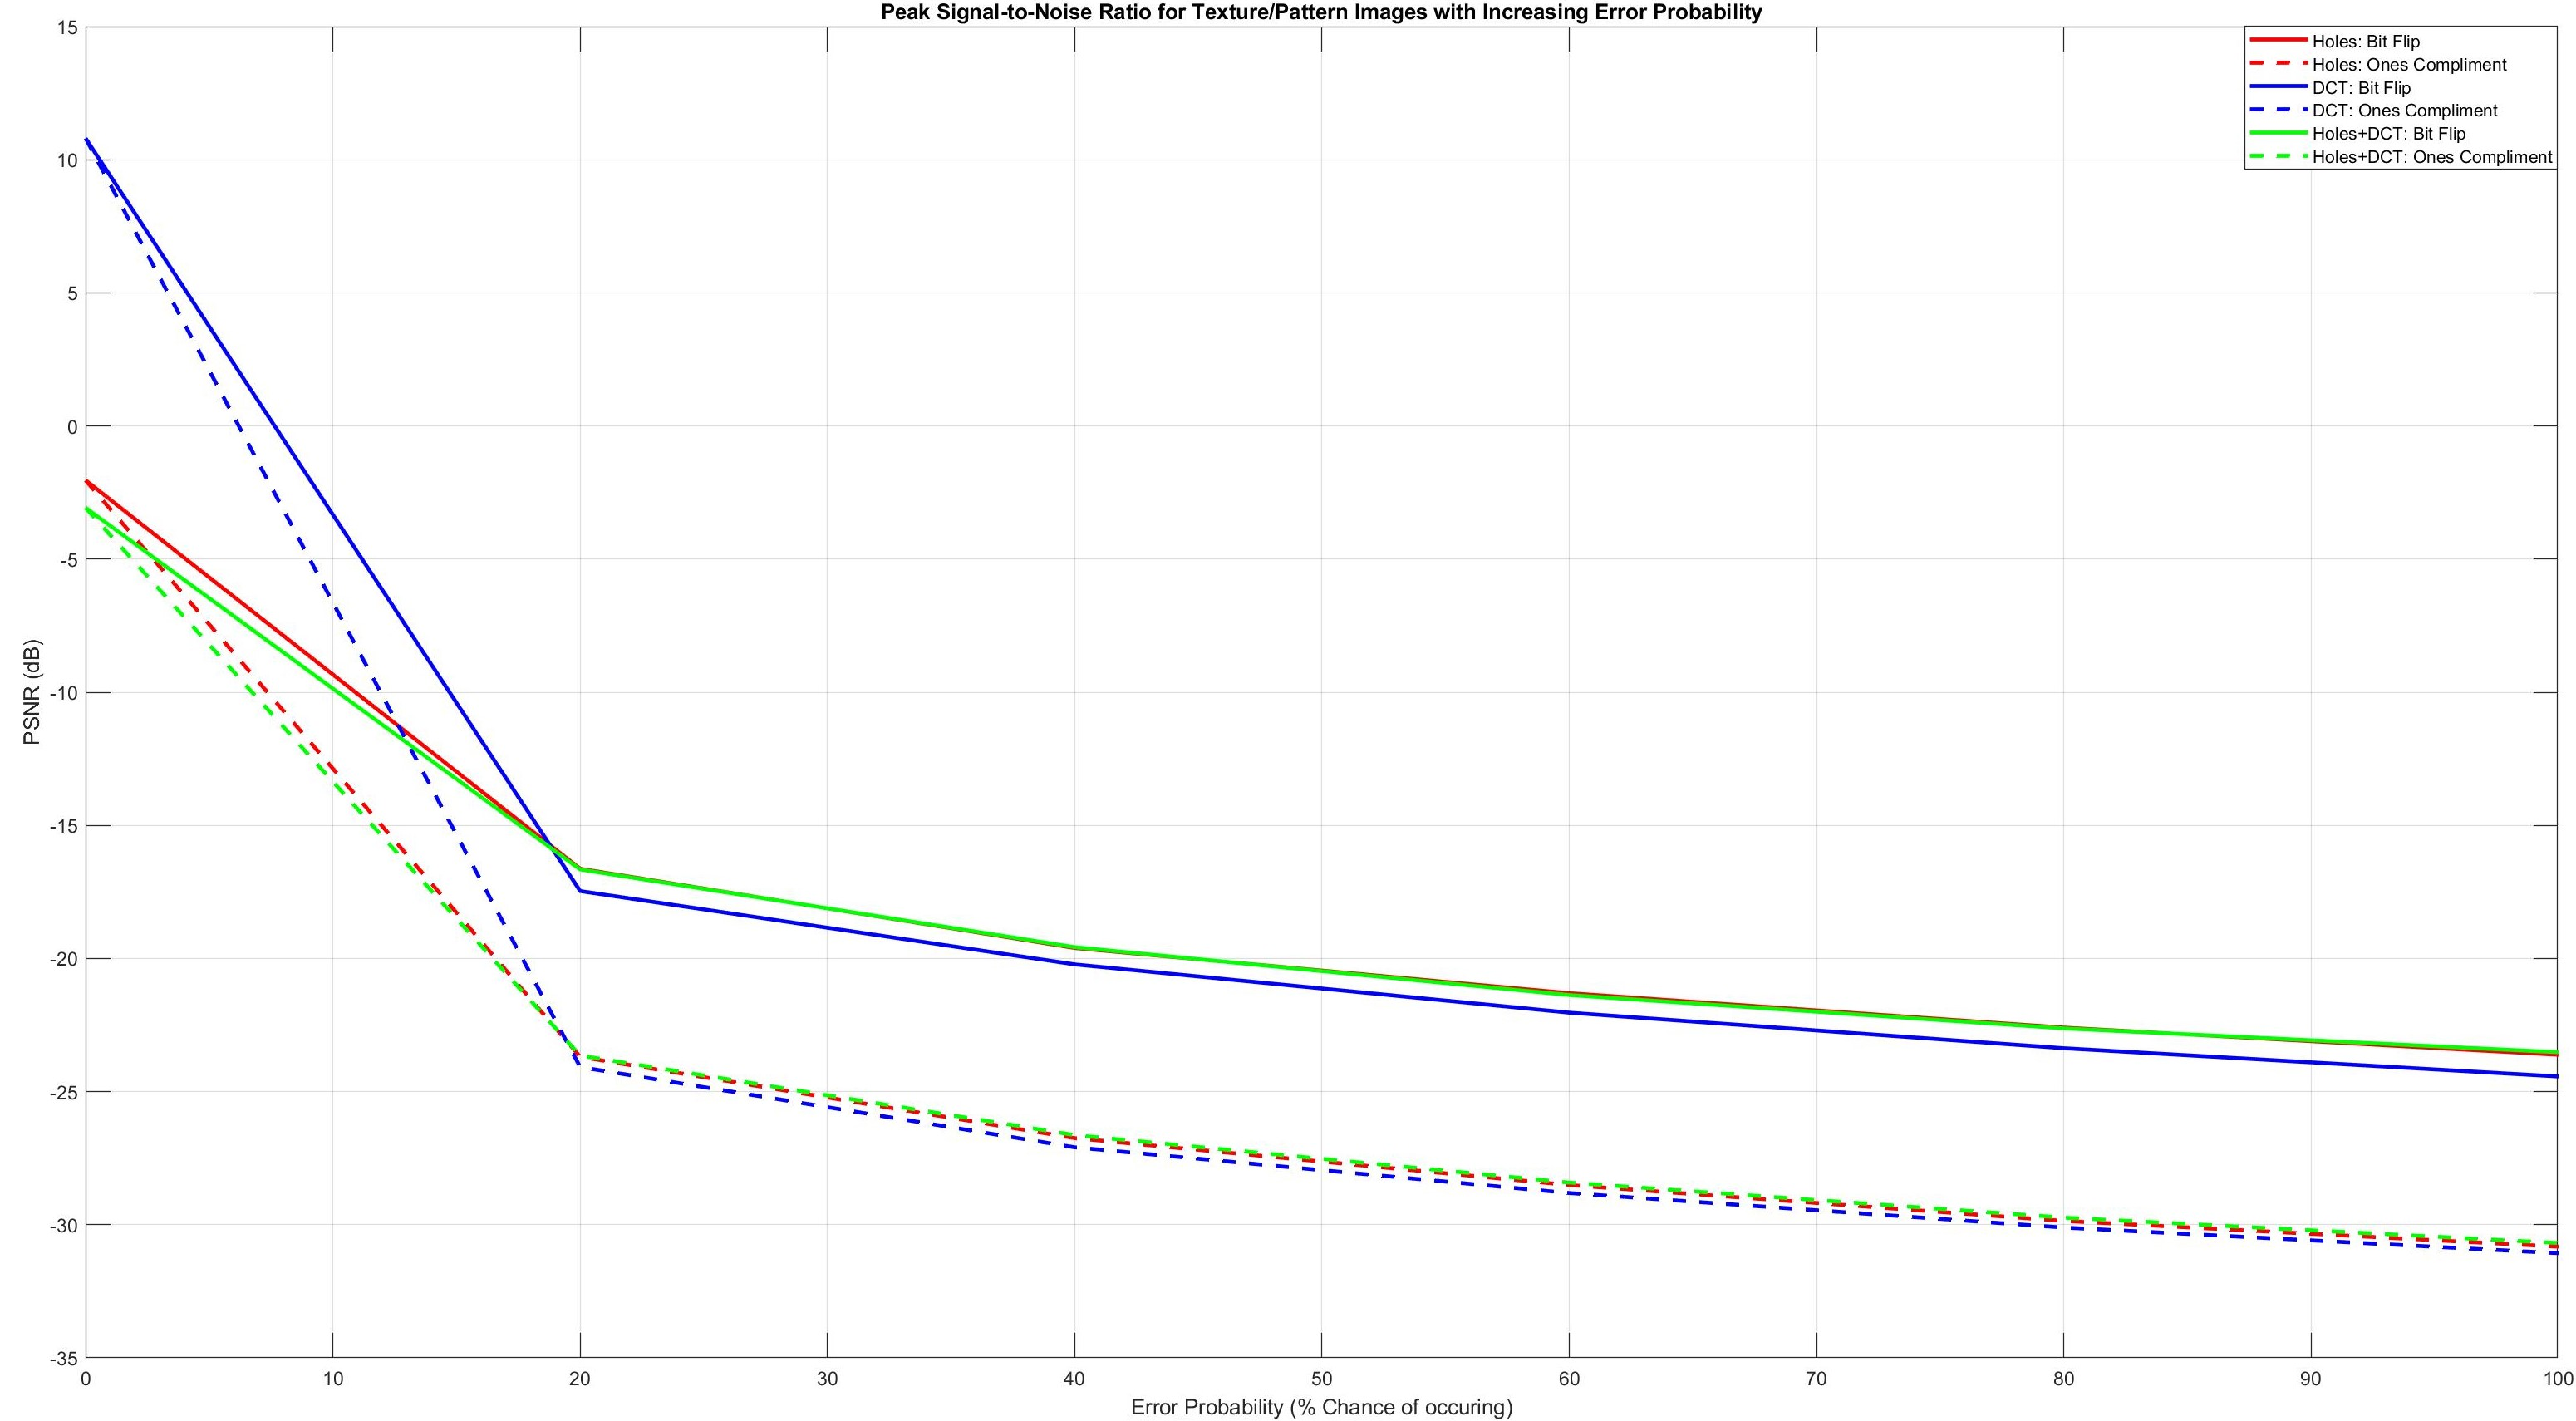
\includegraphics[scale=0.06]{PSNRPattern}
		\caption{PSNR for all Pattern Images} % subcaption
	\end{subfigure}
	\vspace{1em} % here you can insert horizontal or vertical space
	\begin{subfigure}{0.4\textwidth} % width of right subfigure
		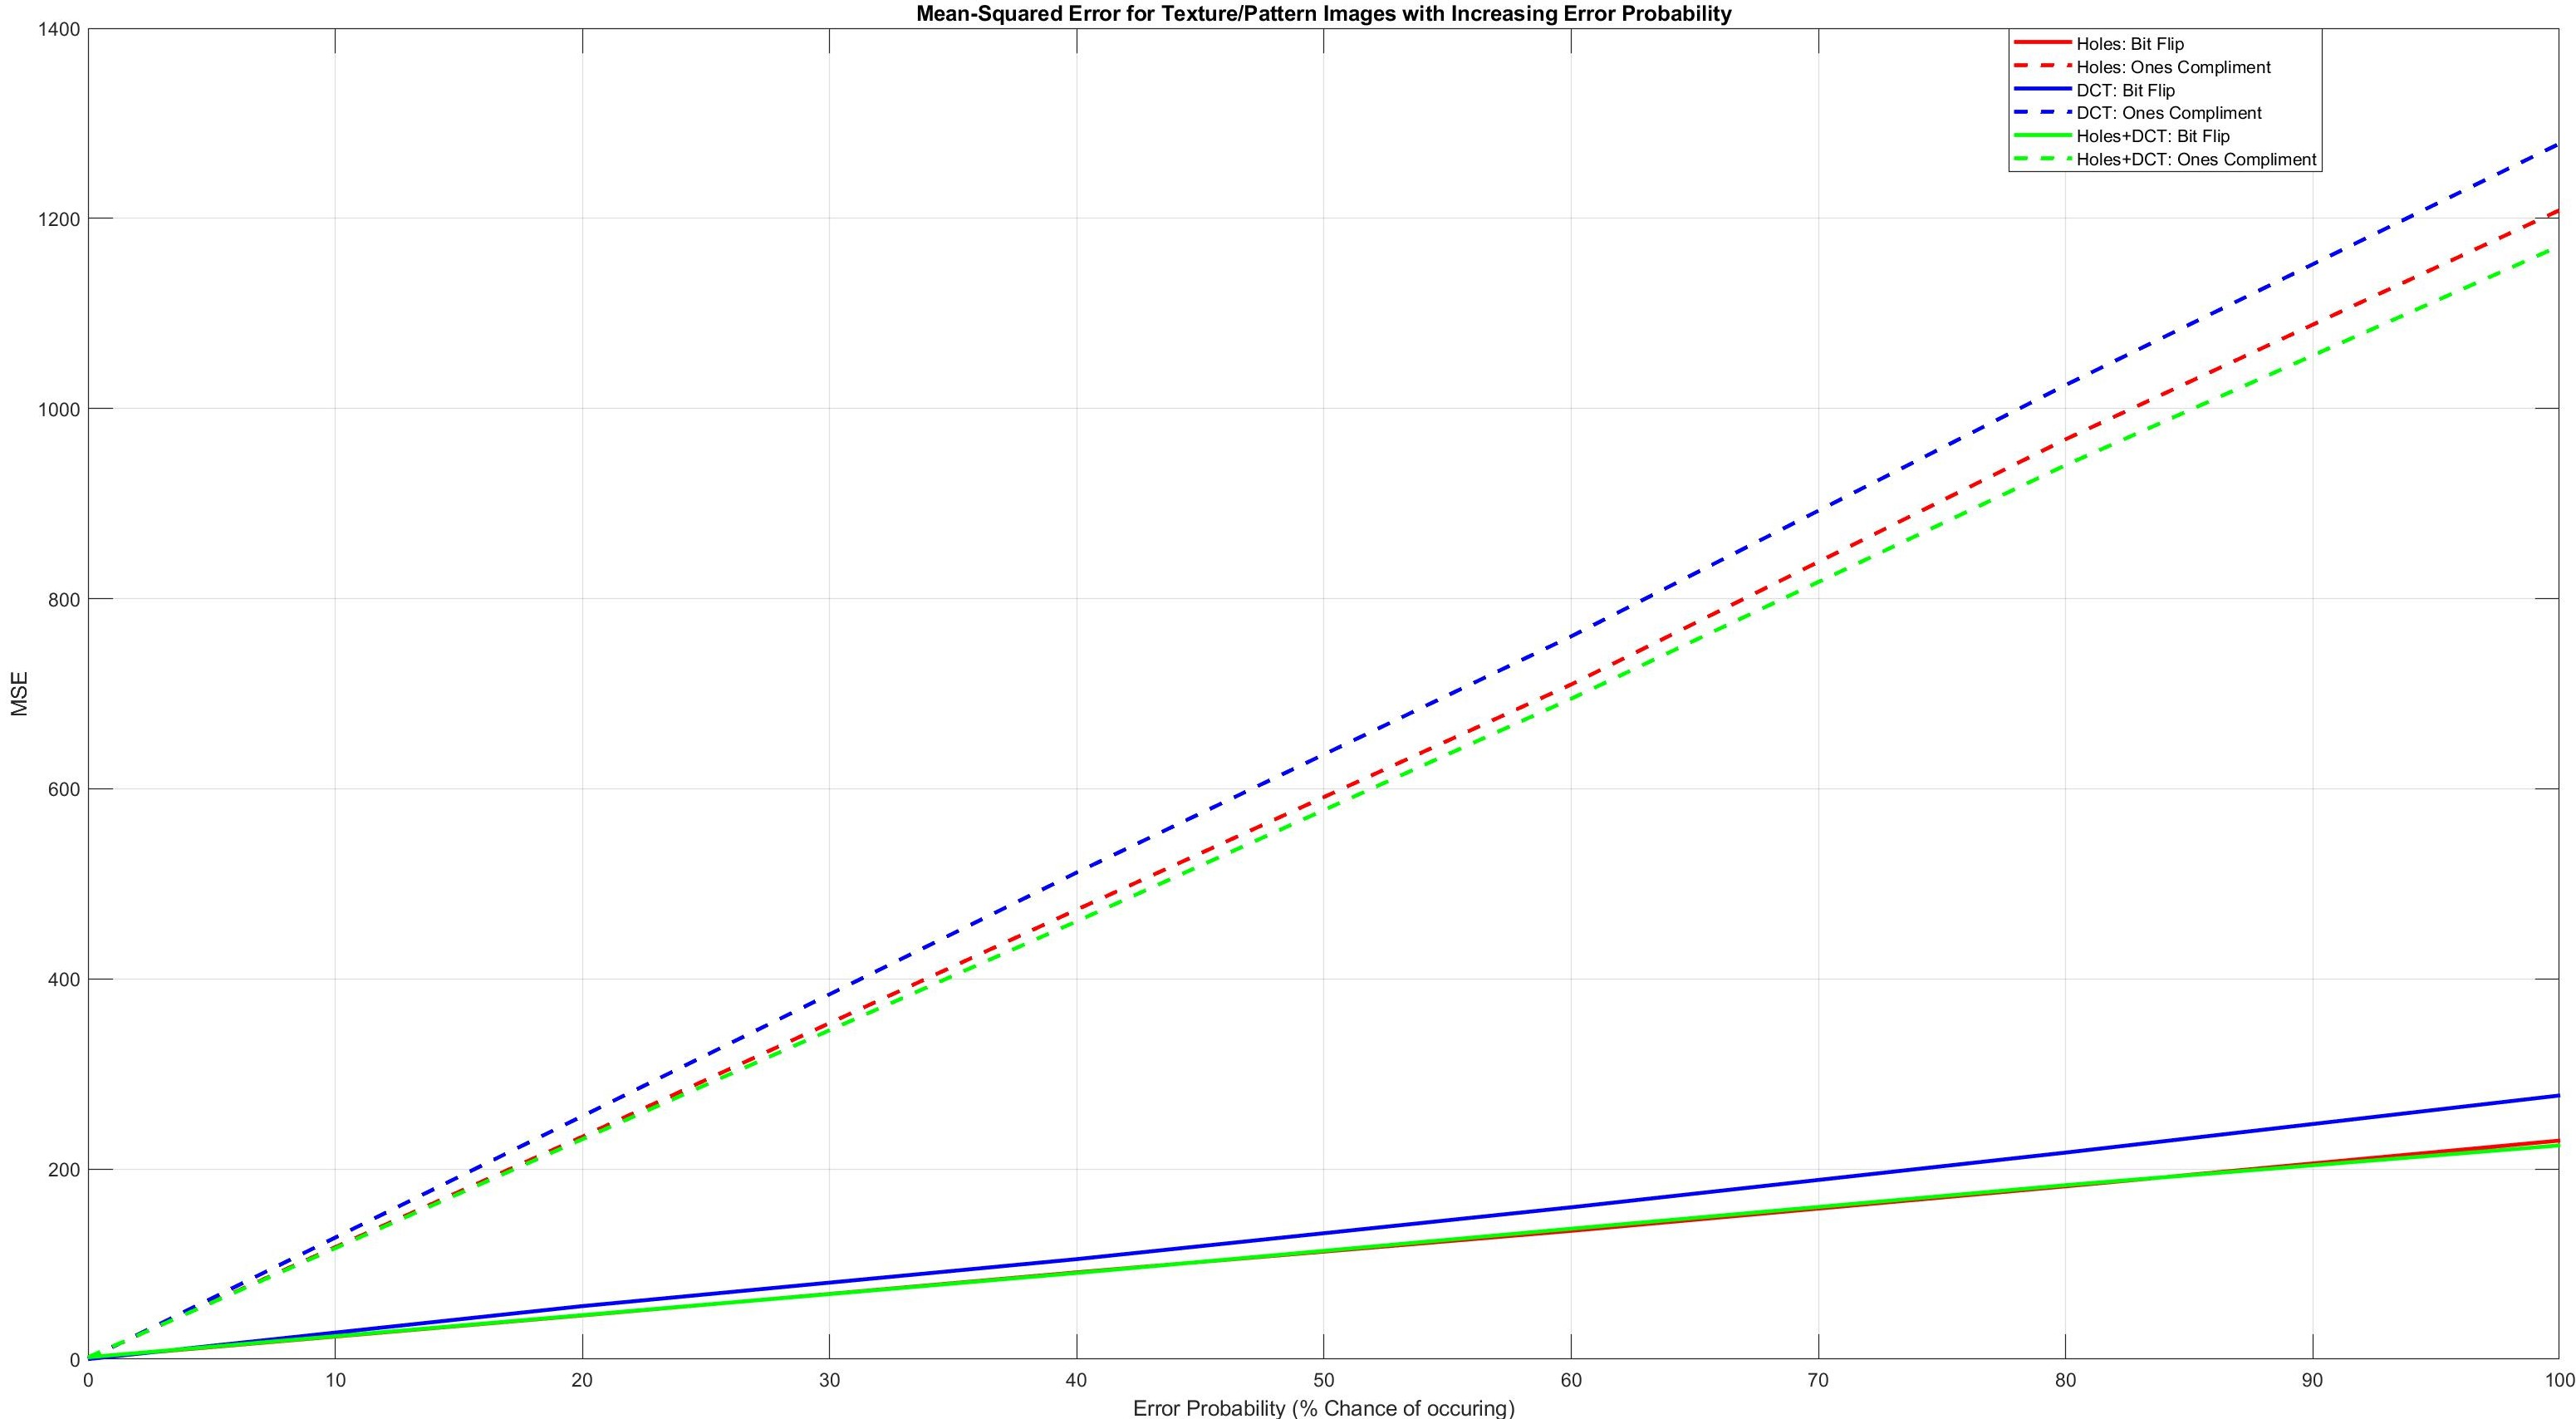
\includegraphics[scale=0.06]{MSEPattern}
		\caption{MSE for all Pattern Images} % subcaption
	\end{subfigure}
	\vspace{-2em}
	\caption{Pattern Images Error Analysis}
	\label{fig: Pattern Error} % caption for whole figure
\end{figure}


\vspace{-1em}
\begin{figure}[H]
\centering
	\begin{subfigure}{0.4\textwidth} % width of left subfigure
		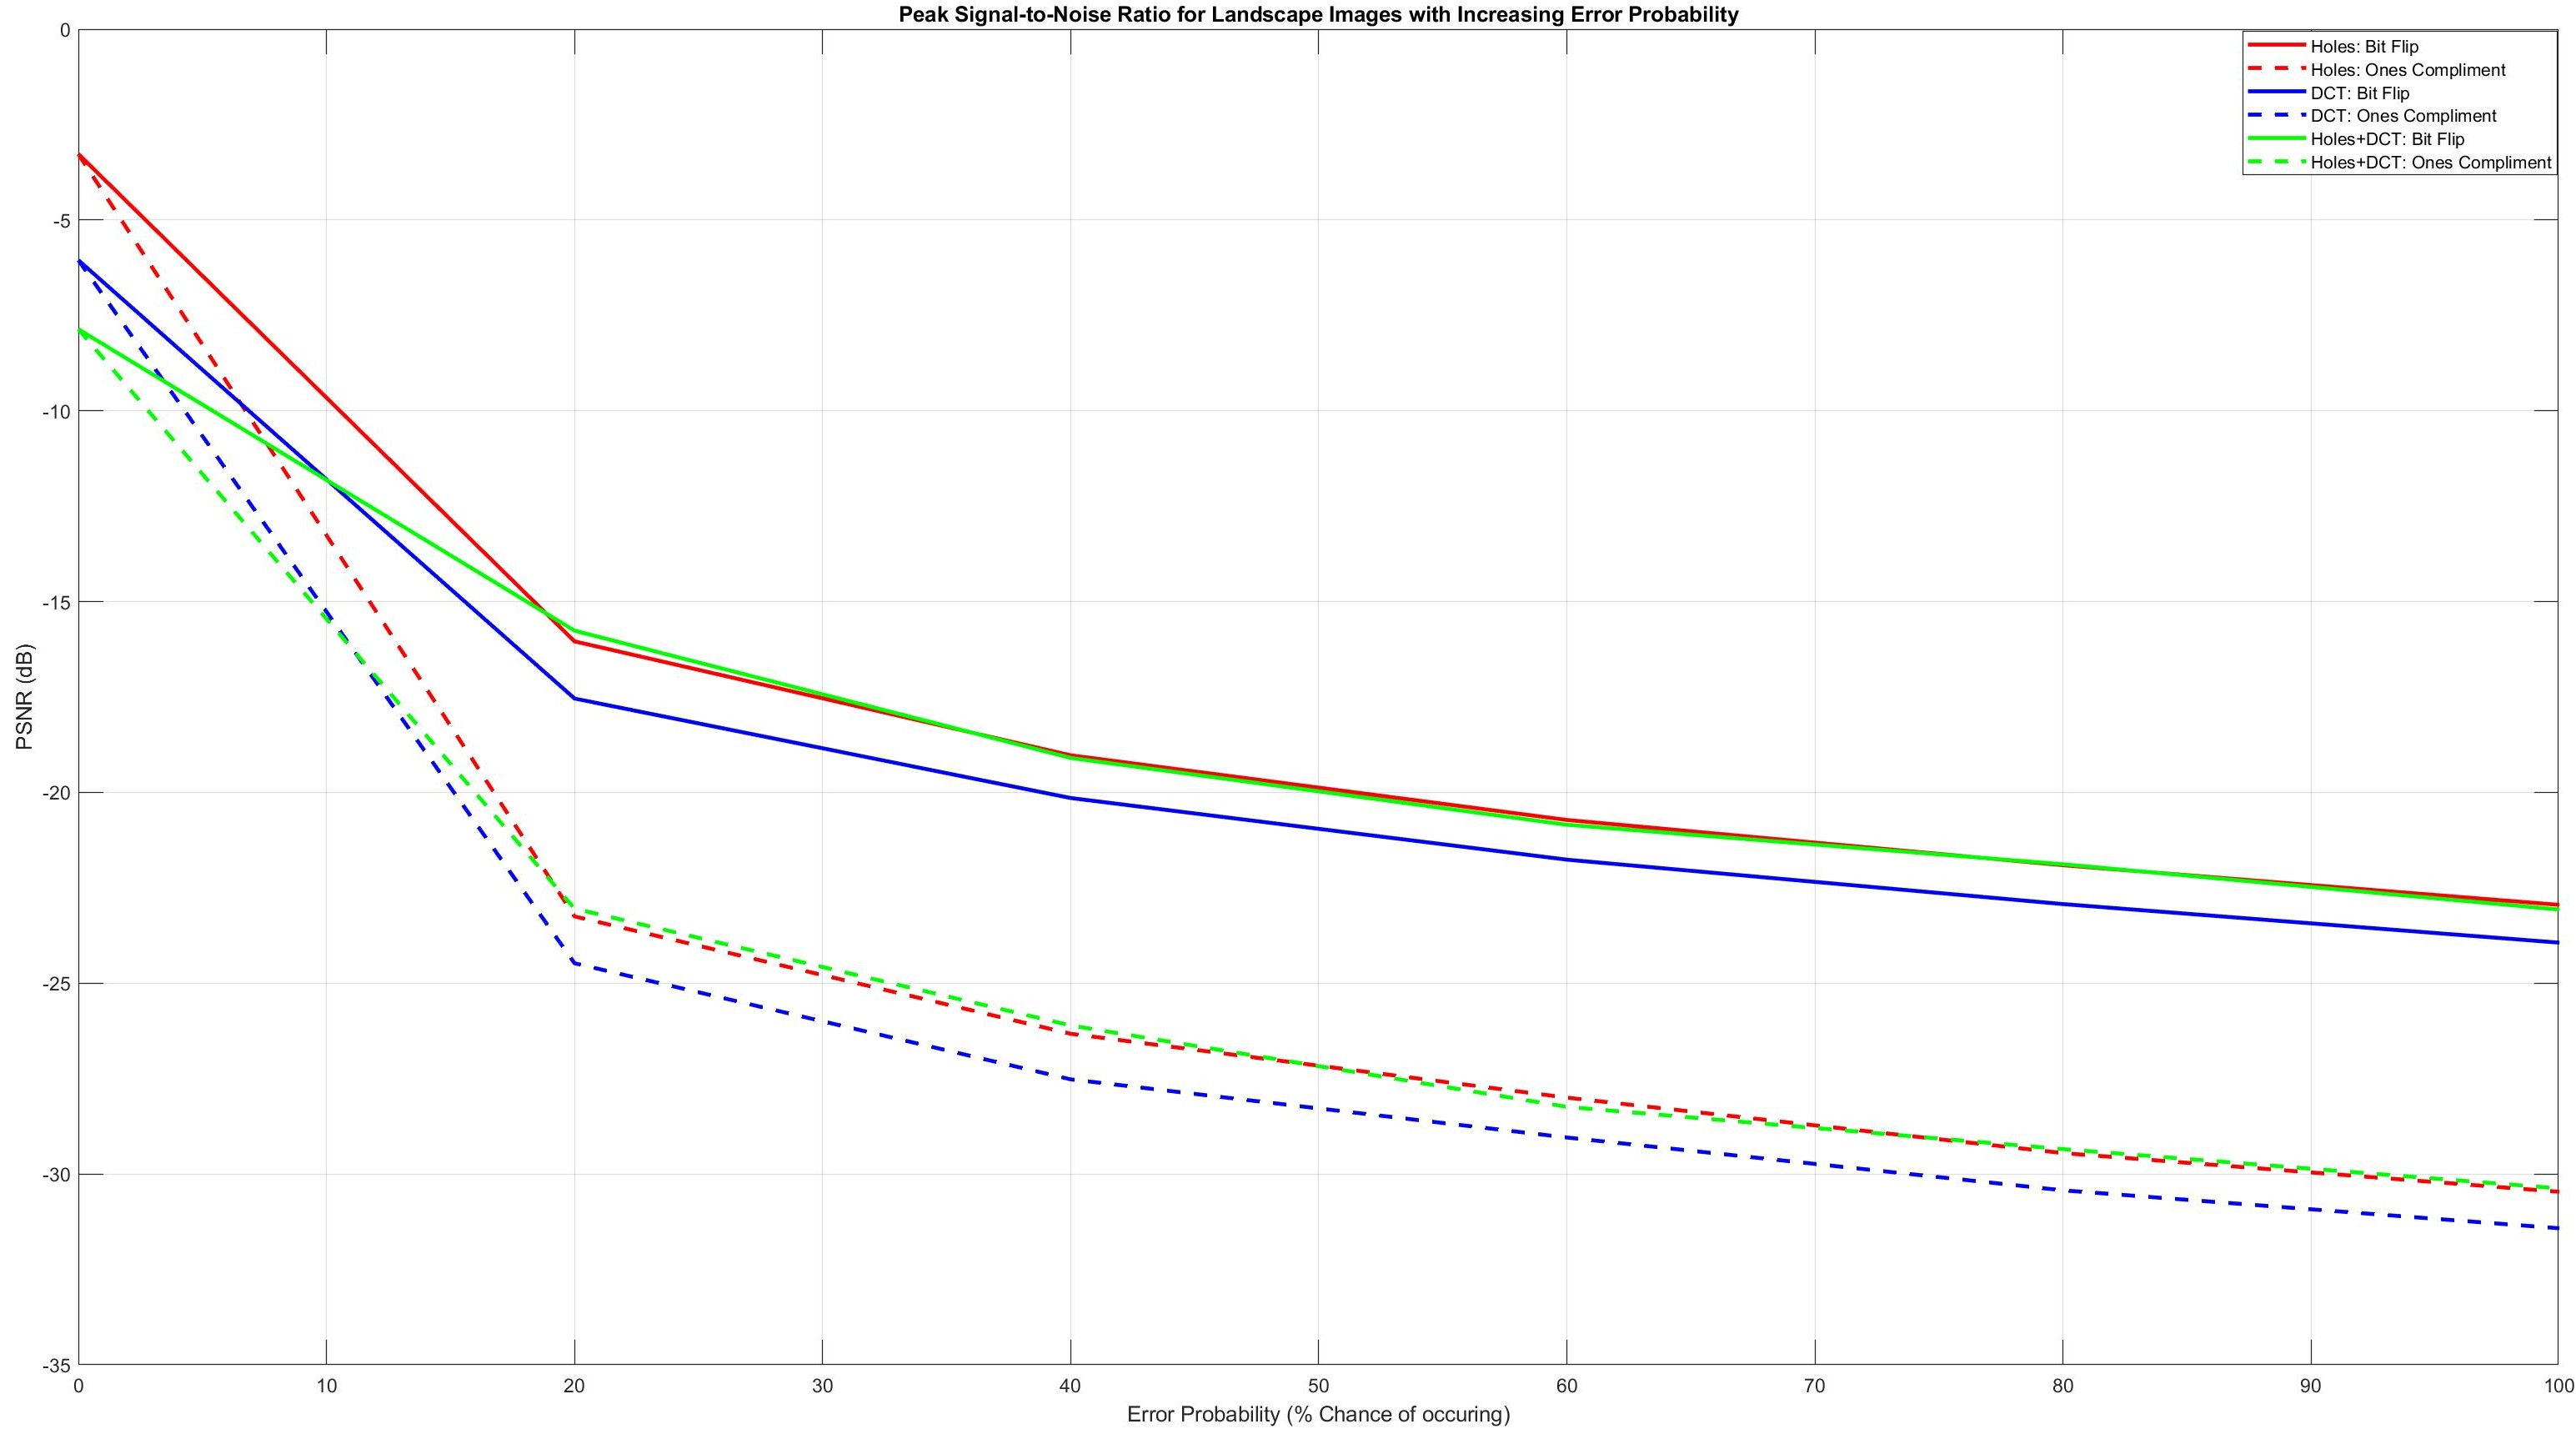
\includegraphics[scale=0.06]{PSNRLandscape}
		\caption{PSNR for all Landscape Images} % subcaption
	\end{subfigure}
	\vspace{1em} % here you can insert horizontal or vertical space
	\begin{subfigure}{0.4\textwidth} % width of right subfigure
		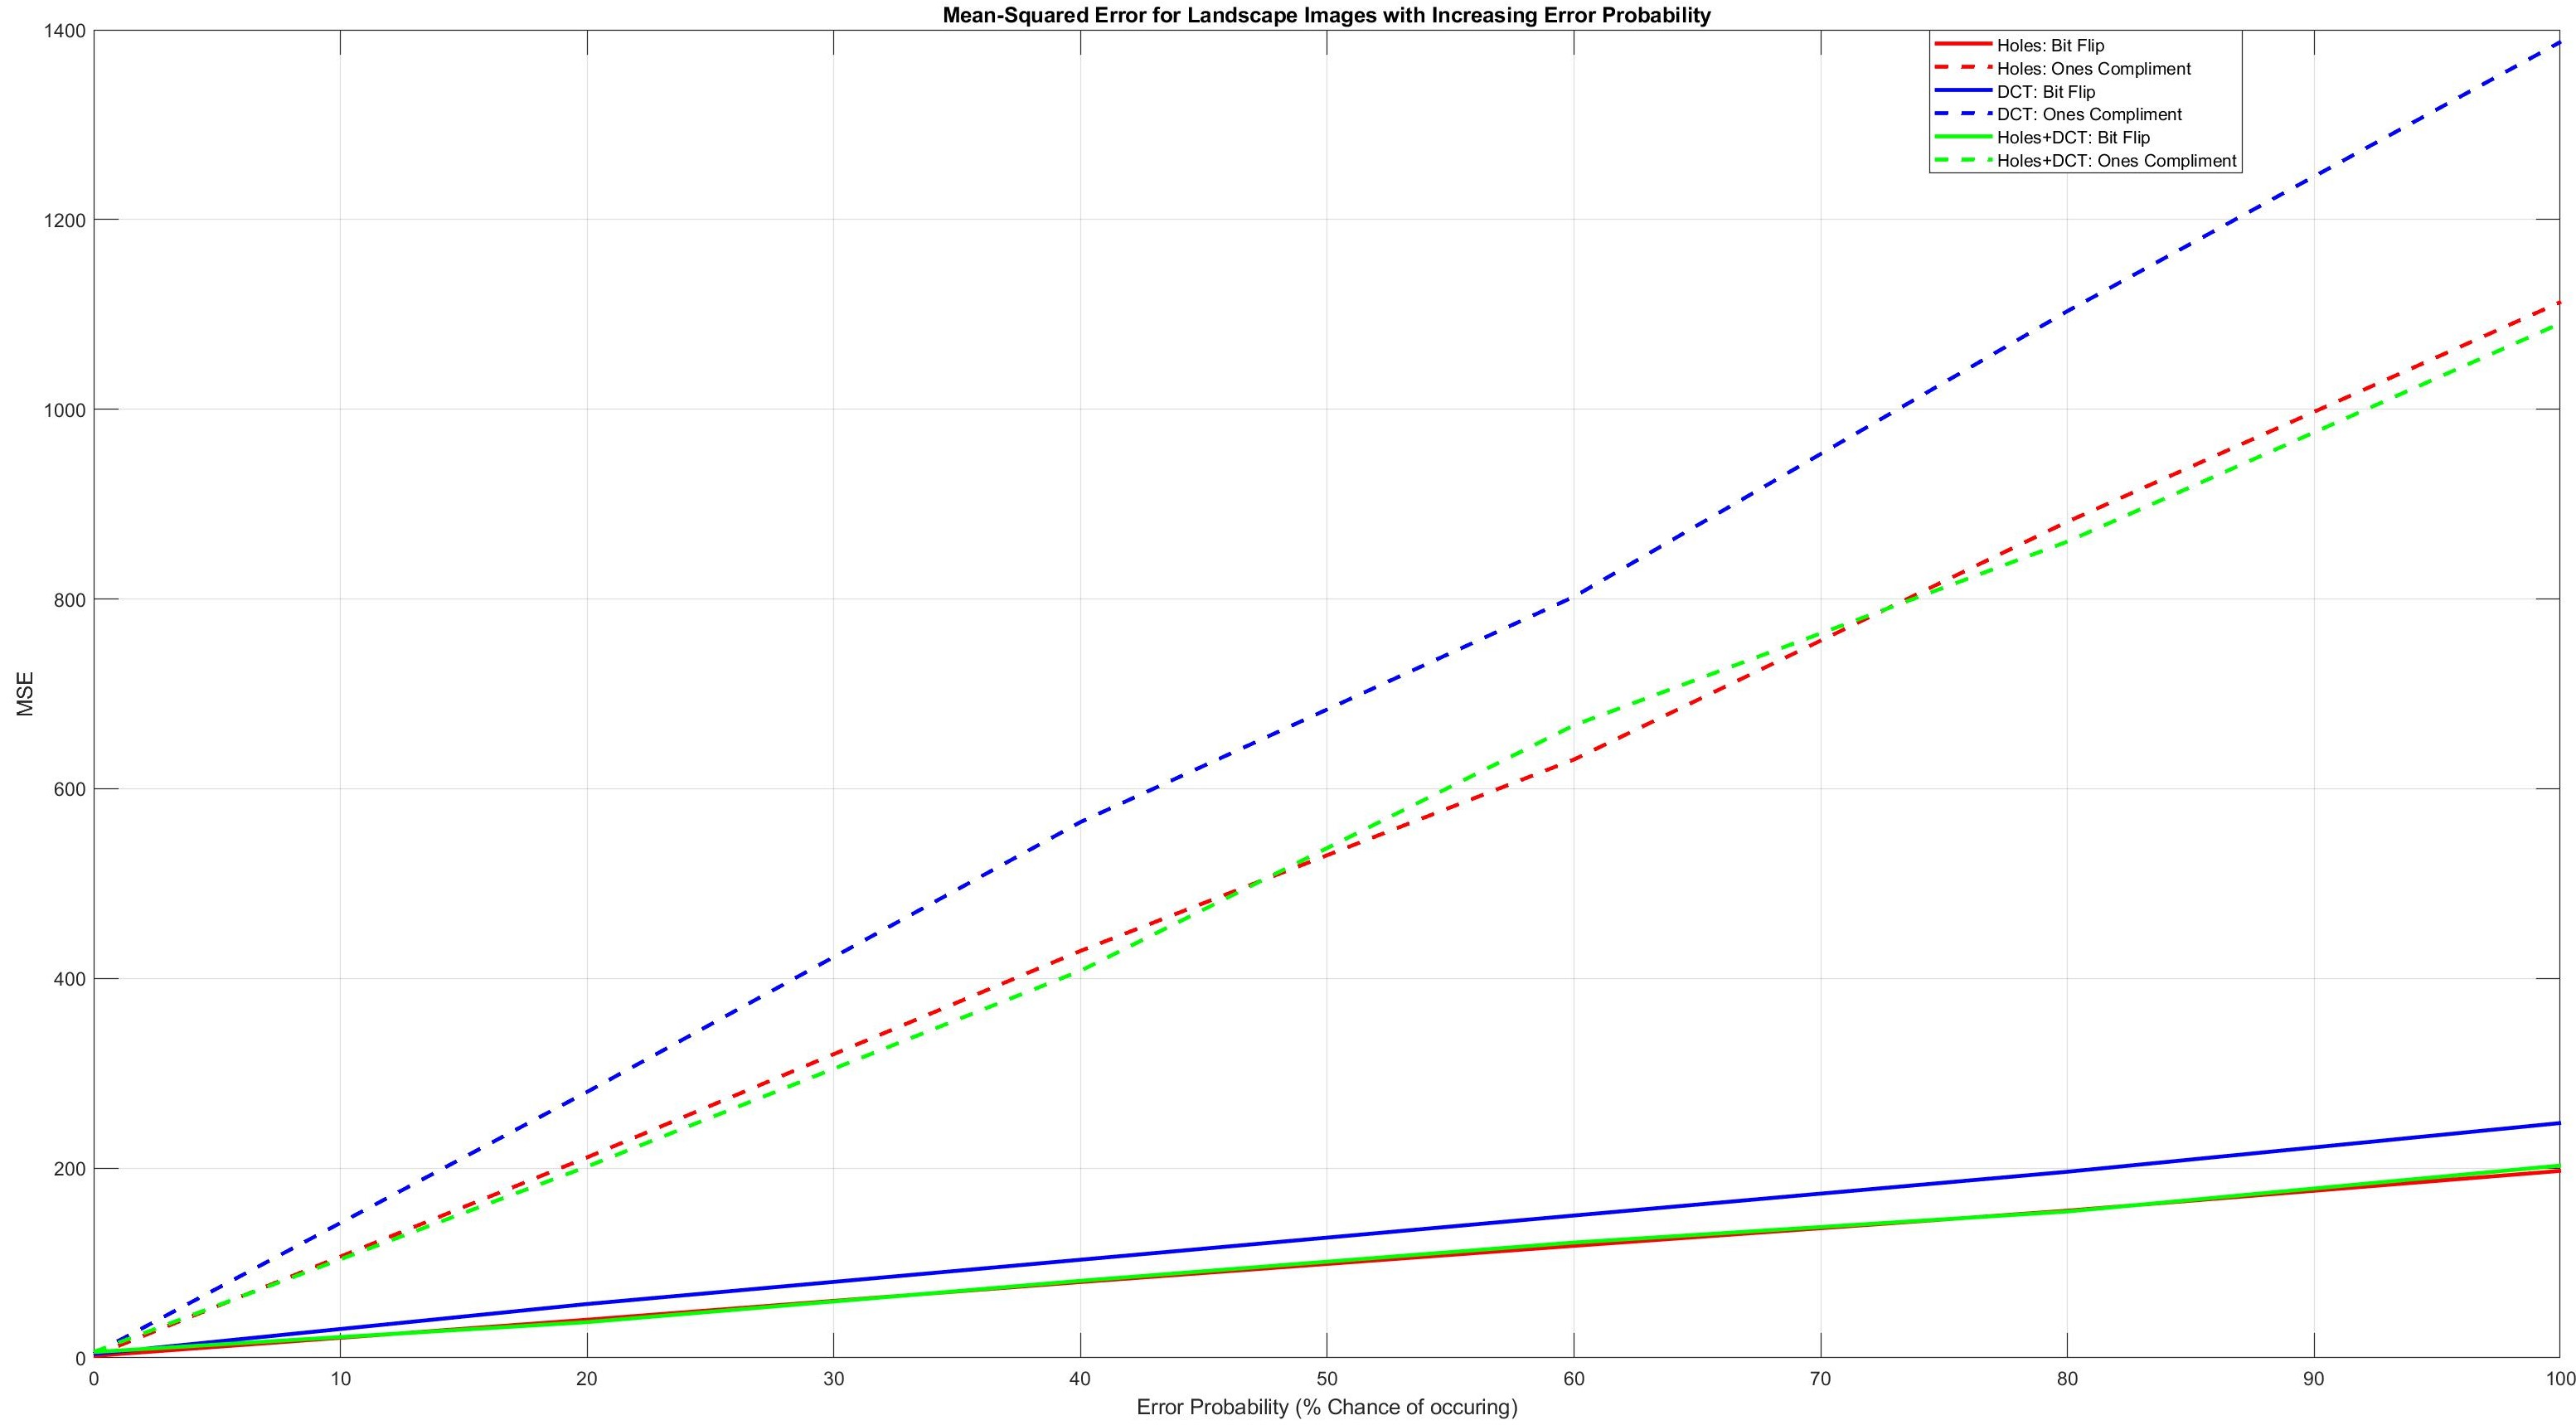
\includegraphics[scale=0.06]{MSELandscape}
		\caption{MSE for all Landscape Images} % subcaption
	\end{subfigure}
	\vspace{-2em}
	\caption{Landscape Images Error Analysis}
	\label{fig: Landscape Error} % caption for whole figure
\end{figure}


\vspace{-1em}
\begin{figure}[H]
\centering
	\begin{subfigure}{0.4\textwidth} % width of left subfigure
		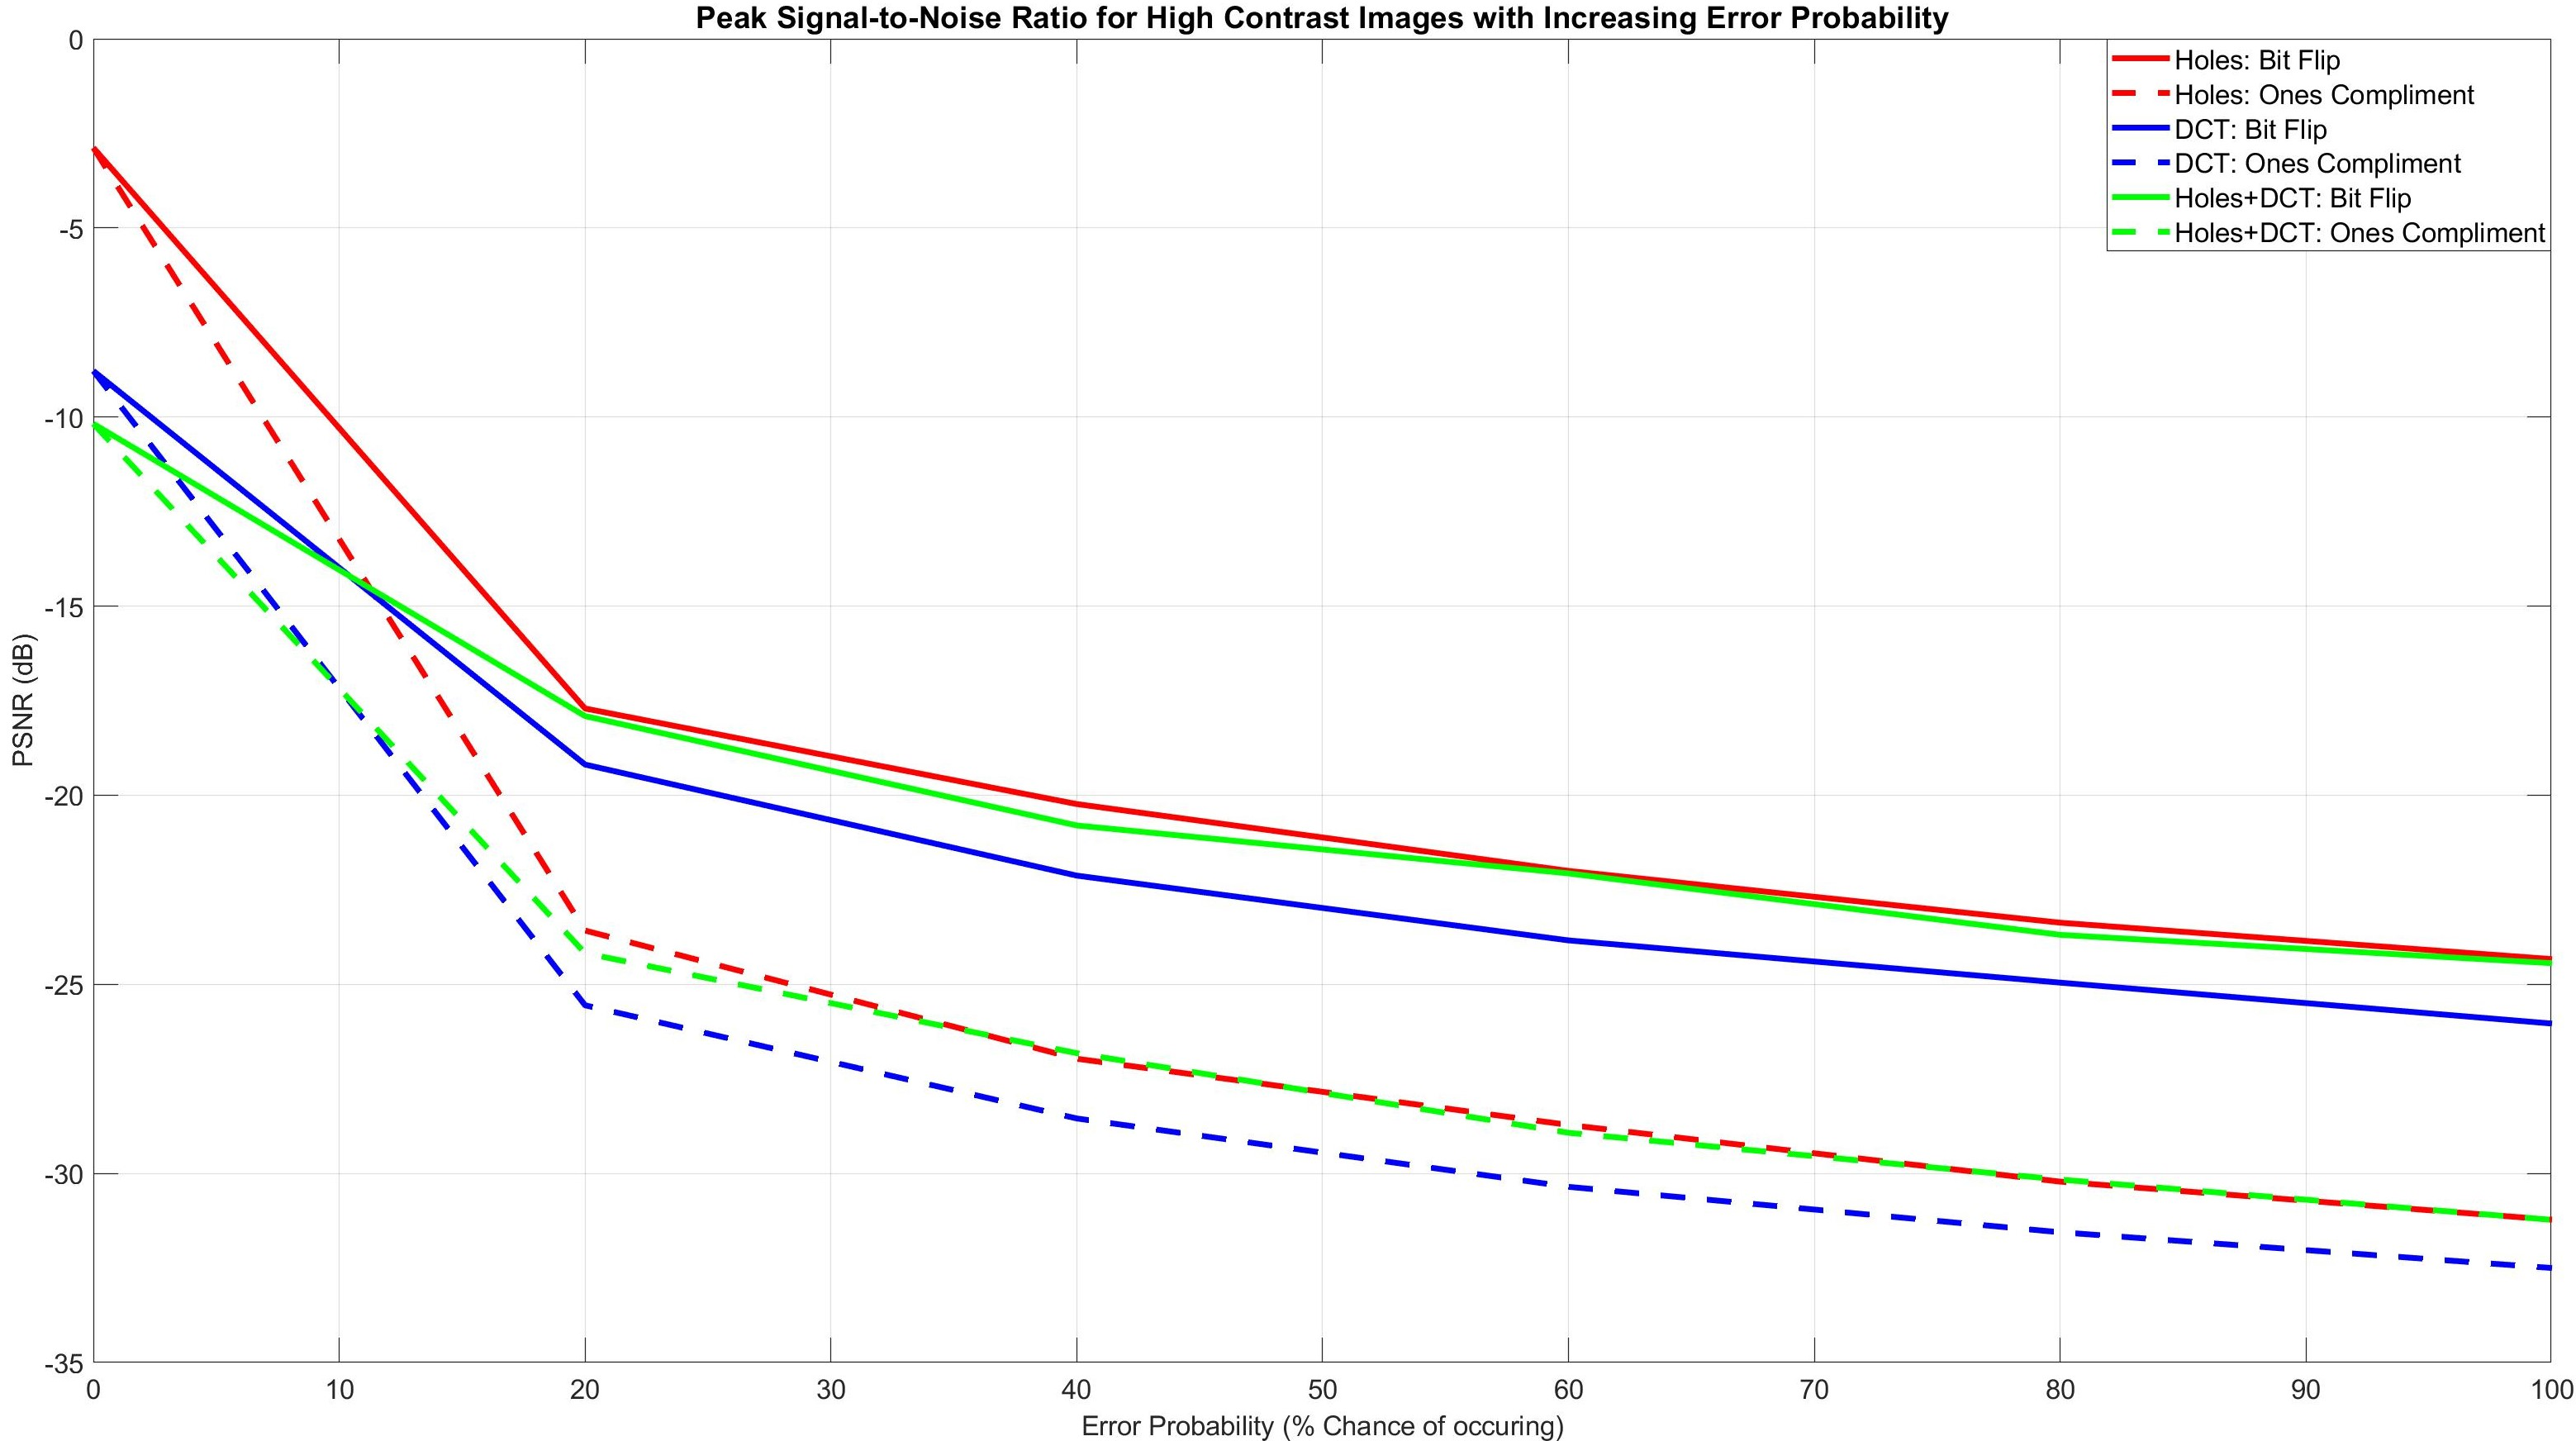
\includegraphics[scale=0.06]{PSNRHigh}
		\caption{PSNR for all High Contrast Images} % subcaption
	\end{subfigure}
	\vspace{1em} % here you can insert horizontal or vertical space
	\begin{subfigure}{0.4\textwidth} % width of right subfigure
		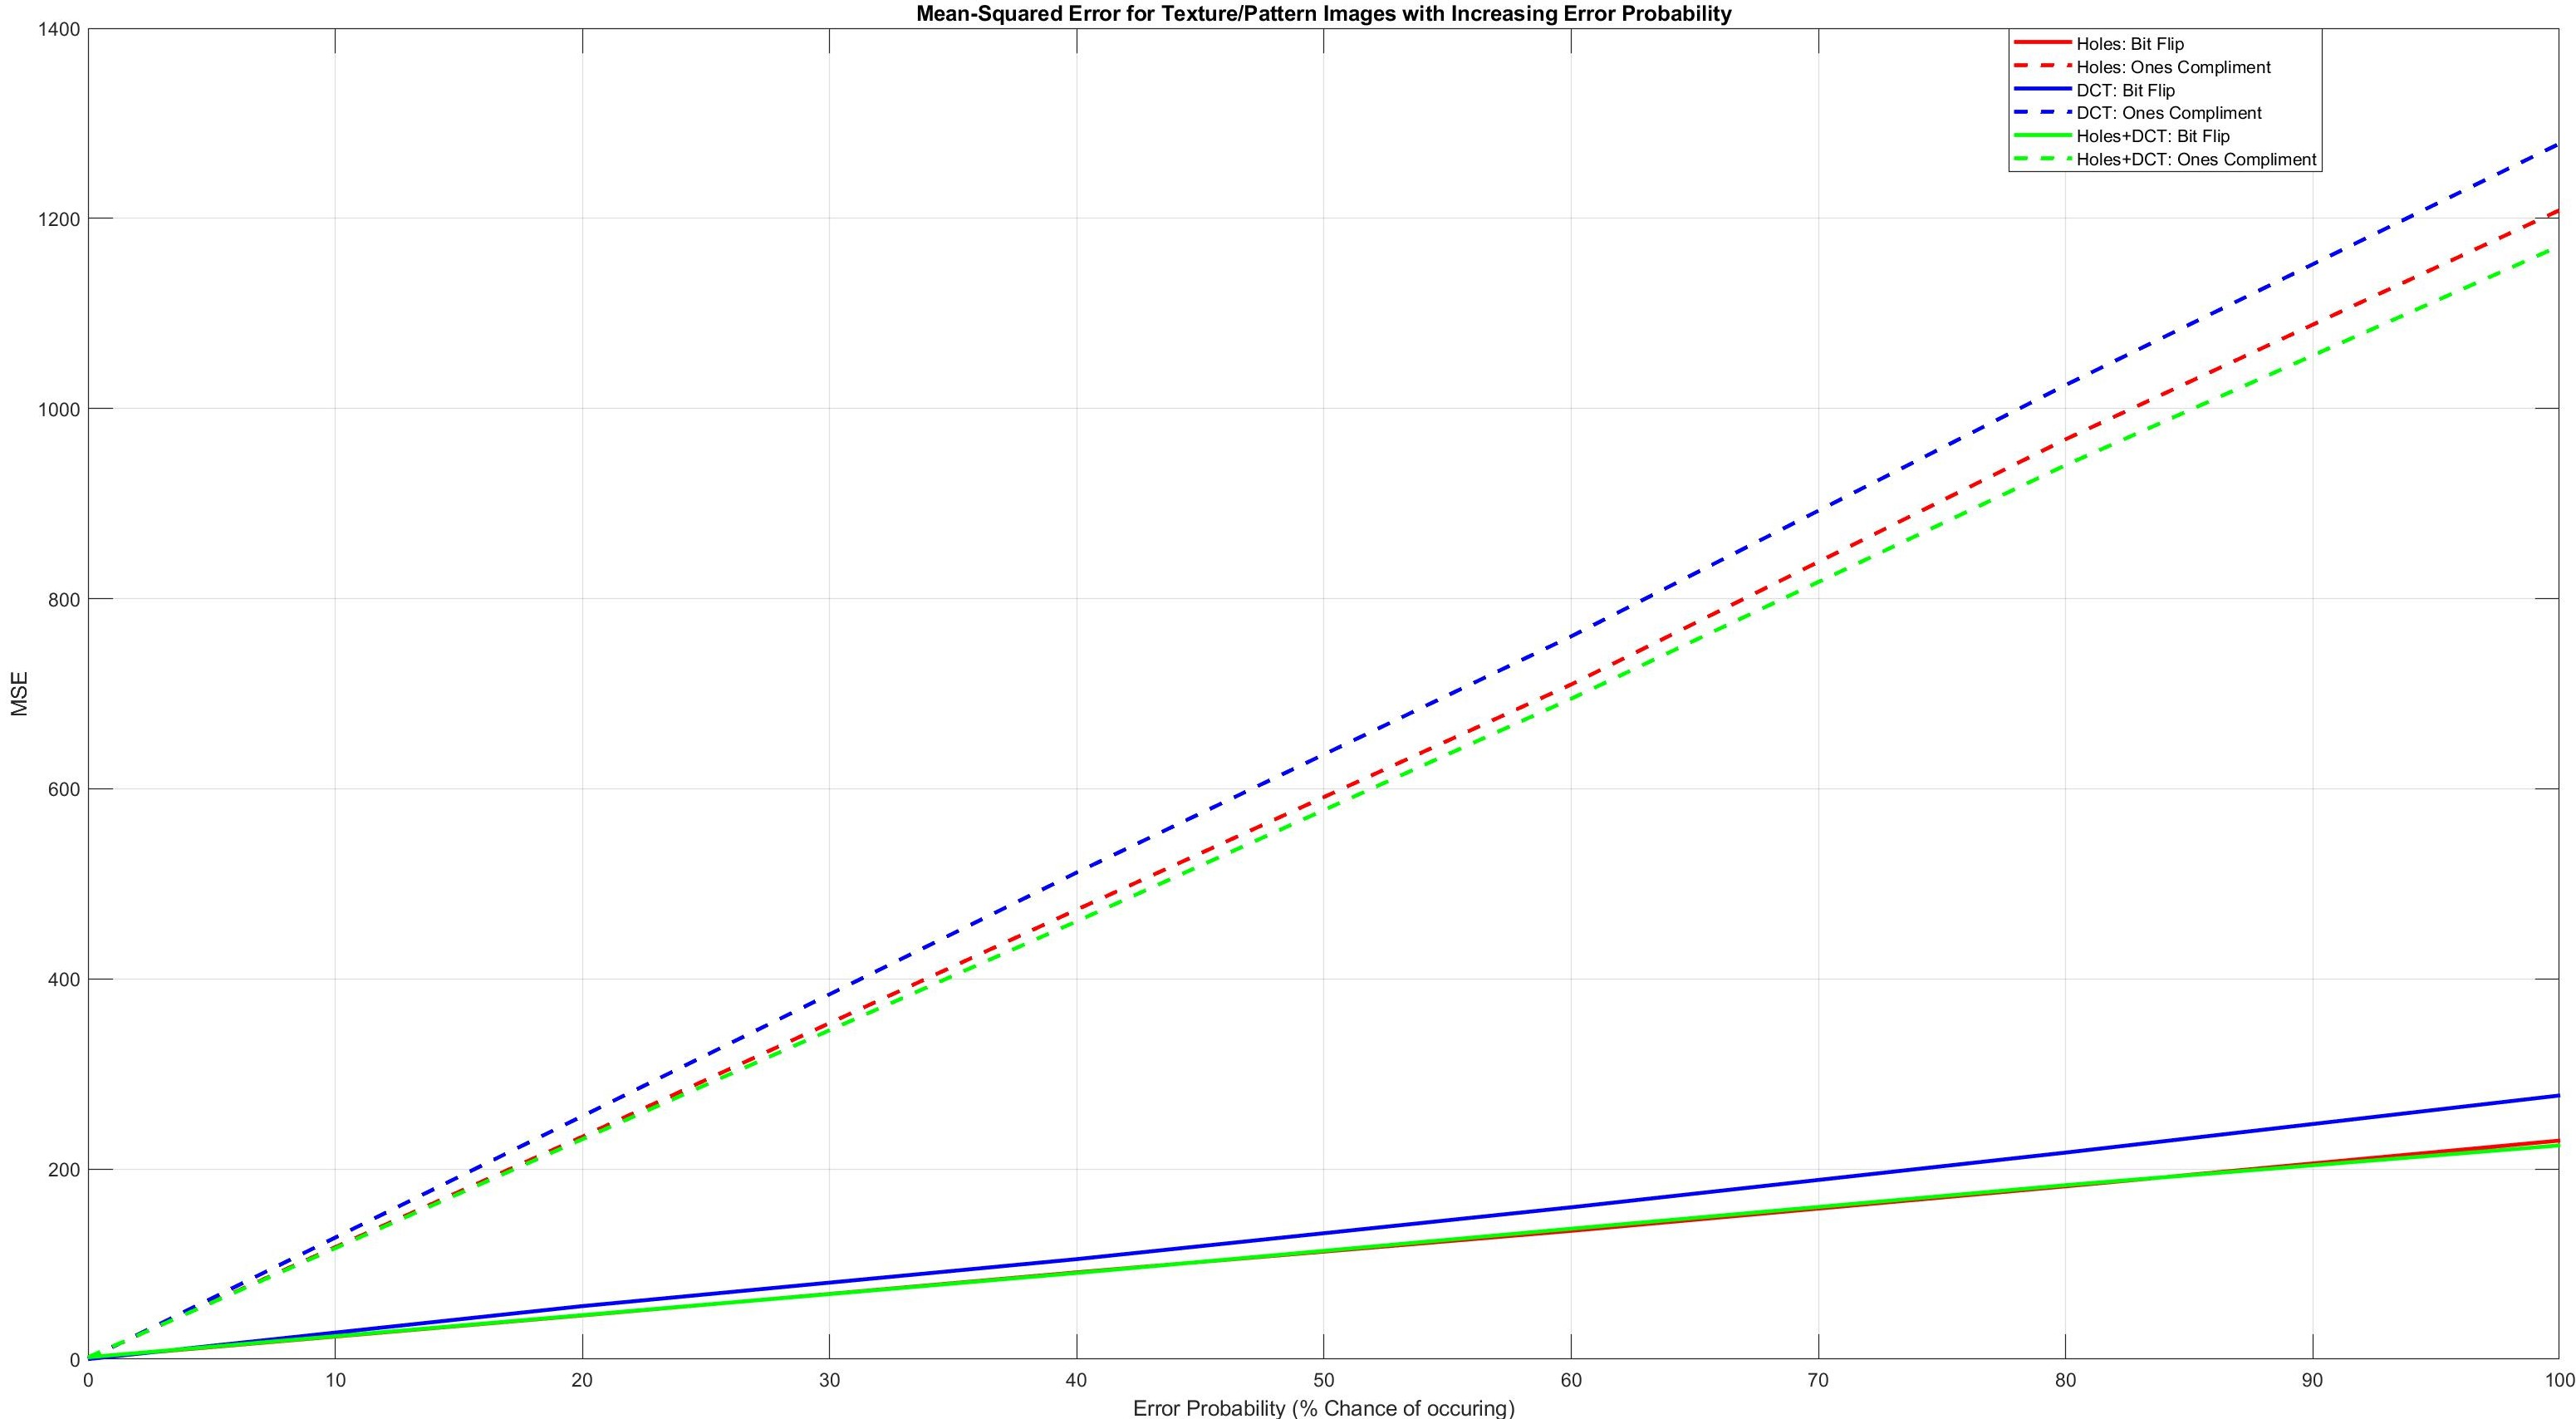
\includegraphics[scale=0.06]{MSEPattern}
		\caption{MSE for all High Contrast Images} % subcaption
	\end{subfigure}
	\vspace{-2em}
	\caption{High Contrast Images Error Analysis}
	\label{fig: High Contrast Error} % caption for whole figure
\end{figure}

	
}

%----------------------------------------------------------------------------------------
%	RESULTS: PROCESSING
%----------------------------------------------------------------------------------------

\headerbox{Results: Processing}{name=resultsProcessing,column=1, above=bottom, below=resultsSimulation}{

}

%----------------------------------------------------------------------------------------
%----------------------------------------------------------------------------------------
%	RIGHT COLUMN
%----------------------------------------------------------------------------------------
%----------------------------------------------------------------------------------------

%----------------------------------------------------------------------------------------
%	FORMULAS
%----------------------------------------------------------------------------------------

\headerbox{Formulas}{name=formulas,column=2,row=0}{
\large \textbf{The Discrete Cosine Transform Formula}
\begin{equation}
\label{eqn: DCT}
\begin{split}
D(i,j) =& \frac{1}{\sqrt{2N}}C(i)C(j)\sum_{x=0}^{N-1}\sum_{y=0}^{N-1}p(x,y) \cos \bigg[ {\frac{(2x+1)i\pi}{2N}}\bigg]\cos \bigg[{\frac{(2y+1)j\pi}{2N}}\bigg]
\end{split}
\end{equation}

\large \textbf{The Chebyshev Distance Formula}
\begin{equation}
\label{eqn: Cheby}
\begin{split}
D(p,q) =& \max_i(|p_i-1_i|)
\end{split}
\end{equation}

\large \textbf{Run Length Encoding}
	\begin{center}\vspace{-3mm}
		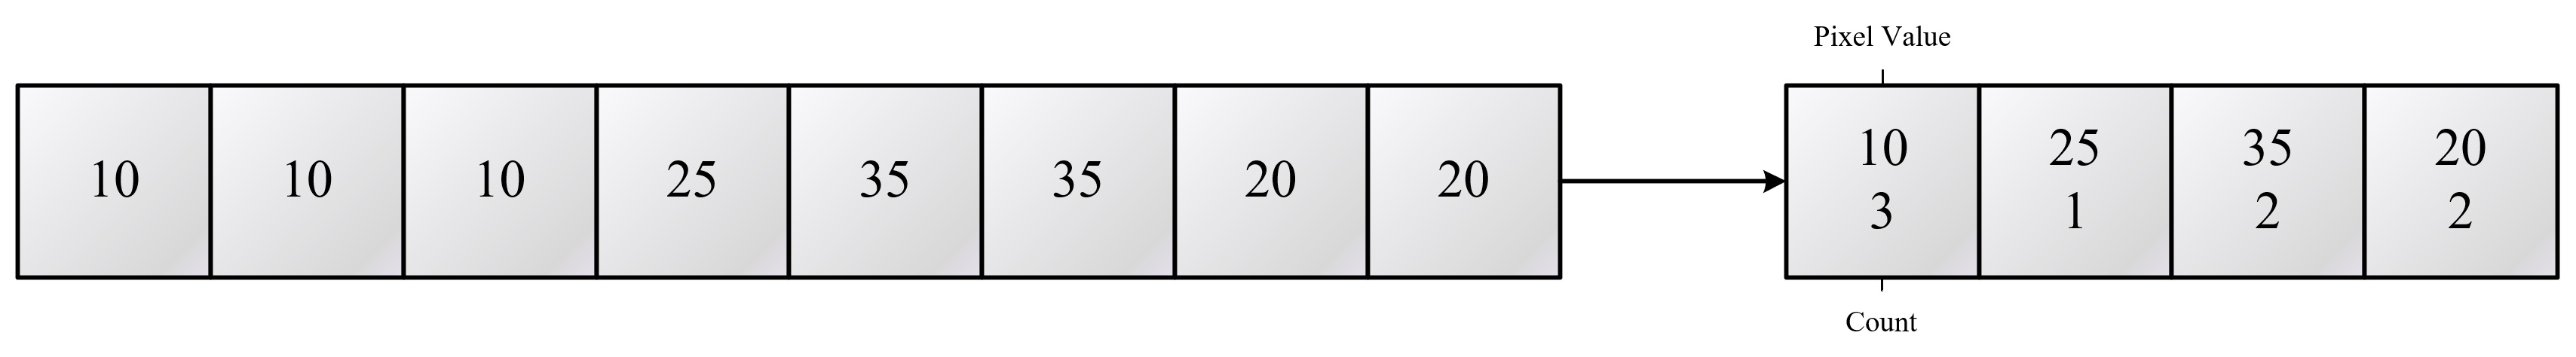
\includegraphics[scale=0.2]{RLE}
	\end{center}
\vspace{-1em}	
\large \textbf{Compression Ratio}
\begin{equation}
\label{eqn: CR}
\begin{split}
CR &= \frac{No.\ of\ bits\ in\ uncompressed\ image}{No.\ of\ bits\ transmitted\ after\ encoding}
\end{split}
\end{equation}

}


%----------------------------------------------------------------------------------------
%	FUTURE WORK
%----------------------------------------------------------------------------------------

\headerbox{Future Work}{name=FutureWork,column=2,below=formulas}{
The designed algorithm for image compression can be improved in numerous ways, including:
\begin{itemize}\compresslist
	\vspace{-0.4em}
	\item Utilizing parallel computing and programming to speed up the processing time of the algorithm
	\item A neural network can be trained on multiple images so that holes can be created in the larger picture as opposed to smaller 8x8 blocks within the image
	\item A neural network trained on multiple images at different compression depths can determine the correct check value
	\item A trained neural network can ultimately reconstruct an image and improve detail and quality of low-quality images.

\end{itemize}
}


%----------------------------------------------------------------------------------------
%	CONCLUSION
%----------------------------------------------------------------------------------------

\headerbox{Conclusion}{name=conclusion,column=2,below=FutureWork}{ % This block's bottom aligns with the bottom of the conclusion block
This project is more research based, and is proof of concept that multiple compression types can be utilized together for image compression. The 


}

%----------------------------------------------------------------------------------------
%	ACKNOWLEGEMENTS
%----------------------------------------------------------------------------------------

\headerbox{Acknowledgements}{name=acknowledgement,column=2,below=conclusion}{ % This block's bottom aligns with the bottom of the conclusion block
The pattern, landscape and high contrast images are taken from \code{Unsplash.com}, and the images used in this poster are by Andrej Lisakov and Pietro De Grandi.\\
The engineers would like to thank Professor Fambirai Takawira for his assistance as supervisor for this project.


}

%----------------------------------------------------------------------------------------
%	REFERENCES
%----------------------------------------------------------------------------------------

\headerbox{References}{name=references,column=2,above=bottom, below=acknowledgement}{
	\renewcommand{\section}[2]{\vskip 0.05em} % Get rid of the default "References" section title
	\nocite{*} % Insert publications even if they are not cited in the poster
\begin{thebibliography}{}
\bibitem{Error}
Uthayakumar, J. et al; \emph{A survey on data compression techniques: From the perspective of data quality, coding schemes, data type and applications}; Journal of King Saud University - Computer and Information Sciences (2018)

\end{thebibliography}
}


%------------------------------------------------



%----------------------------------------------------------------------------------------

\end{poster}

\end{document}